\chapter{Nonlinear model predictive control for steerable wheeled mobile robots}

%\begin{abstract}
%    Steerable wheeled mobile robots (SWMRs) are known to be flexibile and robust thanks to their omnidirectionality and the presence of conventional wheels. Nevertheless, modeling and control of this kind of platform is complex, due to the presence of singularities in their representation or in the control scheme. This paper proposes a framework for trajectory tracking of SWMRs using a Nonlinear Model Predictive Control (NMPC) based on the real-time iteration scheme, which generates feasible motions for the robot by taking into account all kinematic singularities of the mobile base, together with bounds on driving and steering velocities on the wheels. Our NMPC works alongside a finite state machine and an auxiliary trajectory generation module based on dynamic feedback linearization, which makes our framework capable of tracking any trajectory, without ever encountering any singularity. Our approach is validated on a Neobotix MPO-700 on trajectories of increasing difficulty.
%\end{abstract}

\section{Introduction}
Mobile robots equipped with multiple steerable wheels (Fig. \ref{fig:mpo-700}) have greater maneuverability than other wheeled mobile robots, since they are omnidirectional \cite{RobuffoGiordano2009ICRA}. Besides, they can transport higher payloads than omnidirectional robots equipped with mecanum wheels or with omni wheels. Nevertheless, modeling and controlling these robots is not trivial due to the presence of kinematic singularities \cite{Sorour2017RAL}, which need to be handled with particular care, in order to avoid negatively affecting their functionalities.

While many different approaches for modeling and control of steerable wheeled mobile robots (SWMRs) exist in literature, none of them fully exploits their potentialities. The main property of this kind of robots, indeed, is that their instanteneous center of rotation (ICR) can be located anywhere on the plane \cite{Campion1996TR}. This naturally leads to a parametrization based on two-dimensional cartesian \cite{Sorour2016ICRA} or polar coordinates \cite{Connette2008CDC}, which, however, leads to singularities that can make it difficult to develop a control scheme. Sorour et al. \cite{Sorour2017RAL} developed an ICR-based controller which handles singularities of the steering axes. The work is further improved in \cite{Sorour2019RAS}, where the singularity of the ICR at infinity is taken into account through a complementary route strategy. While these approaches consider all singularities of their parametrization, the velocity and acceleration bounds are only considered at the level of the ICR, often resulting in undesired motions with high velocity and high acceleration of the steerable wheels. A singularity-free representation is presented in \cite{Ferland2010IROS} and \cite{Clavien2018EstimationoftheICR}, and used in of~\cite{Clavien2018ICRMotionControl}, where a free-of-singularity motion controller is developed. Here, time scaling is performed to satisfy velocity and acceleration constraints on the wheels, resulting however in non-optimal motion execution.

In this paper, we consider the problem of trajectory tracking for steerable wheeled mobile robots (SWMRs), equipped with an arbitrary number of wheels. The robot is required to follow a user-defined reference pose trajectory in an environment free of obstacles, without violating the driving and steering velocity constraints of each wheel. Note that, in order to successfully perform this task, it is of utmost importance to take into account the kinematic singularities of the platform \cite{Sorour2019RAS}. In order to solve this problem, we propose a Nonlinear MPC \cite{Rawlings2017MPCBook}, which computes control inputs for a SWMR while tracking a reference pose trajectory, satisfying driving and steering velocity constraints on all wheels, and handling all kinematic singularities mentioned above. While there exists a large number of works using MPC on differential drive robots \cite{Tarantos2023Springer}, autonomous vehicles such as cars \cite{Zanon2014Springer} and tractor trailers \cite{Beglini2022TMECH}, and wheeled-legged robots \cite{Bjelonic2021IROS}, the application of MPC to SWMRs has yet to be explored.

%In particular, we present a control scheme for the mobile base of the BAZAR robot \cite{Cherubini2019ACR}, namely the Neobotix MPO-700, which makes use of Nonlinear MPC to safely drive the robot along a reference trajectory, while satisfying all constraints and avoiding singularities. 

\begin{figure}
    \centering
    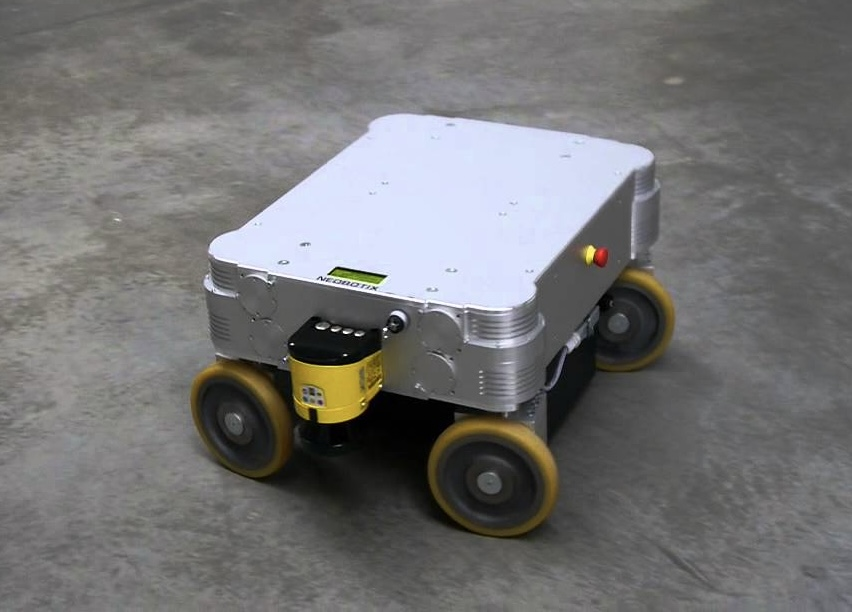
\includegraphics[width=0.7\textwidth]{figures/SWMR/mpo-700.jpg}
    \caption{The Neobotix MPO-700 steerable wheeled mobile robot.}
    \label{fig:mpo-700}
\end{figure}

Our Nonlinear MPC (NMPC) is supported by a finite state machine, which is responsible for starting and stopping the motion of the robot while guaranteeing that the robot never encounters any kinematic singularity, and an auxiliary trajectory generation scheme based on dynamic feedback linearization \cite{Oriolo2002WMRControlDFL}, which generates reference configurations and reference control inputs for the NMPC itself, given a user-defined reference pose trajectory. The NMPC is formulated as a Nonlinear Programming (NLP) problem, and it is solved using the real-time iteration \cite{Gros2020Fromlineartononlinear} scheme.

The contributions of our paper, with respect to the reviewed literature, are the following:
\begin{itemize}
    \item we propose a framework for trajectory tracking of SWMR, which generates motions that satisfy driving and steering velocity bounds on all wheels;
    \item we present a NMPC which is intrinsically free-of-singularities because of the constraints (which guarantees that singularities can never be encountered);
    \item our NMPC is, to the best of our knowledge, the first model predictive control scheme to be applied to a SWMR.
\end{itemize}

Moreover, note that our framework, with respect to the taxonomy of singularities presented in \cite{Sorour2017RAL}:
\begin{itemize}
    \item cannot encounter the singularity of the ICR being on one of the steerable axis because of the NMPC constraints;
    \item cannot encounter singularities due to the mobile base having zero velocity because of the finite state machine (which, as described throughout the paper, makes use of a free-of-singularities kinematic model);
    \item it does not present a singularity when the ICR is at infinity, because of the use of a different parametrization \cite{RobuffoGiordano2009ICRA}.
\end{itemize}  

The paper is structured as follows. Section \ref{sec:kinematic-model} presents the kinematic model of the mobile base, discussing in details the presence of singularities. Section \ref{sec:proposed-framework} introduces the proposed framework, describing the finite state machine (FSM), the auxiliary motion generation scheme, and the NMPC. Section \ref{sec:simulations-and-experiments} validate the proposed framework on multiple experiments, which have been performed using a Neobotix MPO-700. Section \ref{sec:conclusions} concludes the paper, and discusses future works.

\section{Kinematic Model}
\label{sec:kinematic-model}
In this section we will develop the kinematic model of a steerable wheeled mobile robot (SWMR), following the analysis presented in \cite{RobuffoGiordano2009ICRA}. Note that while our mobile base is equipped with azimut wheels (which, in the following, we will denote as steerable wheels), the resulting kinematic model is identical to the one described in the aforementioned paper, which takes into account caster wheels.

Consider a SWMR equipped with $n_s \ge 2$ independent steerable wheels. With reference to Fig. \ref{fig:swmr}, we will denote the vector $\bm{\xi} = [x, y, \theta]^\top \in SE(2)$ as the pose of mobile base, where $(x, y)$ is its position, and $\theta$ is its orientation. Let $S_i$ be the $i$-th steering joint of the mobile base, and $W_i$ be the $i$-th wheel of the mobile base, and let $\bm{o}_{S_i}$ and $\bm{o}_{W_i}$ respectively be their positions, the latter parameterized by the steering angle $\beta_i$. Each wheel is also described by two independent velocities, the driving velocity $v_{Wi}$ and the steering velocity $v_{\beta_i}$, which are taken as control inputs. We define the whole robot configuration via the vector $\bm{q}=[\bm{\xi}^\top, \bm{\beta}^\top]^\top$, where $\bm{\beta}=[\beta_1, \dots, \beta_{n_s}]^\top$.

\begin{figure}
    \centering
    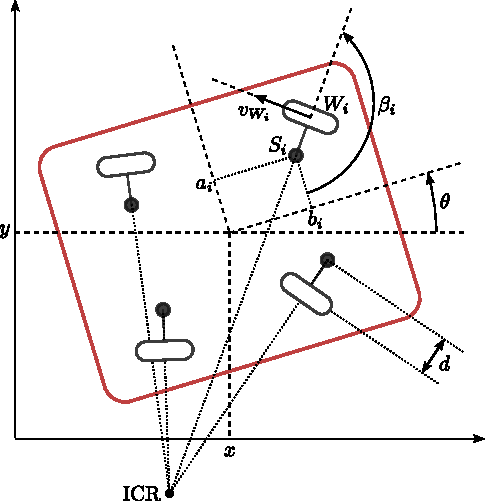
\includegraphics[width=0.65\textwidth]{figures/SWMR/swmr.pdf}
    \caption{Schematic model of a SWMR. Note that, even if the figure represents a robot equipped with four wheels, our approach is generic and works with an arbitrary number of wheels.}
    \label{fig:swmr}
\end{figure}

The position of the $i$-th steering joint $S_i$ is defined as
\begin{align*}
    \bm{o}_{S_i} &=
    \begin{bmatrix}
        x \\
        y
    \end{bmatrix}
    +
    \bm{R}(\theta)
    \begin{bmatrix}
        b_i \\
        a_i
    \end{bmatrix},
\end{align*}
and the position of the $i$-th wheel $W_i$ is defined as
\begin{align*}
    \bm{o}_{W_i} &=
    \bm{o}_{S_i}
    +
    \bm{R}(\theta + \beta_i)
    \begin{bmatrix}
        0 \\
        -d
    \end{bmatrix}.
    %\\&=
    %\begin{bmatrix}
    %    x + b_i \cos\theta - a_i \sin\theta + d \sin(\theta + \beta_i) \\
    %    y + b_i \sin\theta + a_i \cos\theta - d \cos(\theta + \beta_i),
    %\end{bmatrix}
\end{align*}
where $\bm{R} \in SO(2)$ is a rotation matrix.
%while its velocity can be defined by
%\begin{align*} 
%    \dot{\bm{o}}_{W_i} &=
%    \begin{bmatrix}
%        \dot{x} \\
%        \dot{y}
%    \end{bmatrix}
%    +
%    \dot{\bm{R}}(\theta)
%    \begin{bmatrix}
%        b_i \\
%        a_i
%    \end{bmatrix}
%    +
%    \dot{\bm{R}}(\theta + \beta_i)
%    \begin{bmatrix}
%        0 \\
%        -d
%    \end{bmatrix}
%    \\&=
%    \begin{bmatrix}
%        \dot{x} - (b_i \sin\theta + a_i \cos\theta) \dot{\theta} + d \cos(\theta + \beta_i) (\dot{\theta} + \dot{\beta}_i) \\
%        \dot{y} + (b_i \cos\theta - a_i \sin\theta) \dot{\theta} + d \sin(\theta + \beta_i) (\dot{\theta} + \dot{\beta}_i)
%    \end{bmatrix}.
%\end{align*}

Due to the assumption of no lateral skidding (i.e., the velocity of the contact point of the wheel must be orthogonal with respect to the zero motion line of the wheel itself), each wheel is subject to the Pfaffian constraint
\begin{equation}
    \label{eq:no-lateral-skidding-constraint}
    \begin{bmatrix}
        -\sin(\theta + \beta_i) \\
         \cos(\theta + \beta_i)
    \end{bmatrix}^\top \dot{\bm{o}}_{W_i} = 0.
\end{equation}
%which can be rewritten as
%\begin{equation}
%    \label{eq:no-lateral-skidding-constraint}
%    -\sin(\theta + \beta_i) \dot{x} +
%    \cos(\theta + \beta_i) \dot{y} +
%    (b_i \cos(\beta_i) + a_i \sin(\beta_i)) \dot{\theta} = 0.
%\end{equation}

By combining the above equations, it is possible to rearrange the $n_s$ nonholonomic constraints in matrix form
\begin{equation}
    \label{eq:pfaffian-constraints-matrix-form}
    \underbrace{
    \begin{bmatrix}
        -\sin(\theta + \beta_1) &
        \cos(\theta + \beta_1) &
        \Delta_1 &
        0 \dots 0 \\
        -\sin(\theta + \beta_2) &
        \cos(\theta + \beta_2) &
        \Delta_2 &
        0 \dots 0 \\
        \vdots & \vdots & \vdots & \vdots \\
        -\sin(\theta + \beta_{n_s}) &
        \cos(\theta + \beta_{n_s}) &
        \Delta_{n_s} &
        0 \dots 0 \\
    \end{bmatrix}
    }_{\bm{A}^\top(\bm{q})}
    \dot{\bm{q}} = 0,
\end{equation}
with $\Delta_i = b_i \cos\beta_i + a_i \sin\beta_i$.

In order for the mobile base to perform a motion, all wheel axles must instantaneously intersect at the same point, the ICR. The existence of an ICR can be seen as a geometric constraint, which requires all wheel orientations to be coordinated. In the following, we will study how the ICR constraint affect the mobility of the system.

\subsection{ICR constraint not satisfied}
Whenever the robot configuration is such that it has no instantaneous center of rotation (ICR), since from~(\ref{eq:pfaffian-constraints-matrix-form}) $\dot{\bm{q}} \in \mathcal{N}(\bm{A}^\top(\bm{q}))$, the kinematic model of the robot is the following:
\begin{align*}
\begin{split}
%    \dot{x} &= 0 \\
%    \dot{y} &= 0 \\
%    \dot{\theta} &= 0 \\
    \dot{\beta}_i &= v_{\beta_i},
\end{split}
\end{align*}
with $v_{\beta_i}$ steering velocities. In this case, the pose of the robot remains constant, and it is only possible to control the steering angles. 

\subsection{ICR constraint satisfied}
\label{sec:icr-constraint-satisfied}
Whenever the robot configuration is such that there exists an ICR, it is possible to simplify~\eqref{eq:pfaffian-constraints-matrix-form} through the use of coordinating functions for $\beta_i$ \cite{RobuffoGiordano2009ICRA}, with $i \ge 2$. The idea is to let the ICR be defined by the trajectory of $\bm{\xi}$, namely $\bm{\xi} \left( t \right)$. Indeed, considering the $i$-th constraint in \eqref{eq:pfaffian-constraints-matrix-form} and solving\footnote{Note that $\beta_i$ could be either $h_i(\bm{\xi}, \dot{\bm{\xi}})$ or $h_i(\bm{\xi}, \dot{\bm{\xi}}) + \pi$. In our analysis, to keep the notation simpler, we consider only the first case. However, when implementing the coordinating function, both cases need to be carefully taken into account.} for $\beta_i$ yields the coordinating function (holonomic constraint)
\begin{equation}
    \label{eq:coordinating-function-pre-kinematic-model}
    \beta_i = h_i(\bm{\xi}, \dot{\bm{\xi}}) = \mathrm{arctan} \frac{-\sin\theta\dot{x}+\cos\theta\dot{y}+b_i\dot{\theta}}{\cos\theta\dot{x}+\sin\theta\dot{y}-a_i\dot{\theta}},
\end{equation}
which can be used to ``transform'' the last $n_s-1$ constraints of \eqref{eq:pfaffian-constraints-matrix-form}, obtaining:
\begin{equation}
    \label{eq:reduced-pfaffian-constraints-matrix-form}
    \begin{bmatrix}
        -\sin(\theta + \beta_1) &
        \cos(\theta + \beta_1) &
        \Delta_1 &
        0
    \end{bmatrix}
    \begin{bmatrix}
        x \\ y \\ \theta \\ \beta_1
    \end{bmatrix}
    = 0,
\end{equation}
\begin{equation*}
    \beta_i = h_i(\bm{\xi}, \dot{\bm{\xi}}), \quad i = 2, \dots, n_s.
\end{equation*}

From \eqref{eq:reduced-pfaffian-constraints-matrix-form}, it is trivial to get the reduced kinematic model
\begin{equation}
\label{eq:reduced-kinematic-model}
\begin{split}
    \dot{x} &= v_{W_1} \cos(\theta + \beta_1) + \omega (b_1 \sin\theta + a_1 \cos\theta) \\
    \dot{y} &= v_{W_1} \sin(\theta + \beta_1) + \omega (-b_1 \cos\theta + a_1 \sin\theta) \\
    \dot{\theta} &= \omega \\
    \dot{\beta}_1 &= v_{\beta_1},
\end{split}
\end{equation}
which can be used together with \eqref{eq:coordinating-function-pre-kinematic-model} to express $\beta_i$ as
\begin{equation}
    \label{eq:coordinating-function-post-kinematic-model}
    \beta_i = h_i(v_{W_1}, \omega, \beta_1) = \mathrm{arctan} \frac{v_{W_1}\sin\beta_1+\omega(b_i-b_1)}{v_{W_1}\cos\beta_1+\omega(a_1-a_i)}.
\end{equation}

Note that the above equations (named \textit{coordinating functions}) present a singularity whenever the position of the $i$-th steering joint $S_i$ is constant (i.e., $\dot{\bm{o}}_{S_i}=\bm{0}$). This needs to be considered when designing a controller. Note that this condition is met when the platform is not moving or when the position of the ICR coincides with the position of $S_i$. 

As a consequence, if the ICR does not lie on any of the steering joints $S_i$ and if it does not change through time (i.e. $\dot{\beta}_i = 0$), all coordinating functions $h_i$ are free of singularity. Two interesting cases when these hypotheses hold are when the ICR is constant at infinity (i.e., $\omega = 0$), and when the ICR is constant, but not at infinity (i.e., $v_{W_1} = \omega R$, with $R > 0$ the distance between $\bm{o}_{W_1}$ and the ICR). In the following, we define the reduced kinematic models and the coordinating functions for these two cases, which will be used to start/stop the robot.

\begin{figure*}
    \centering
    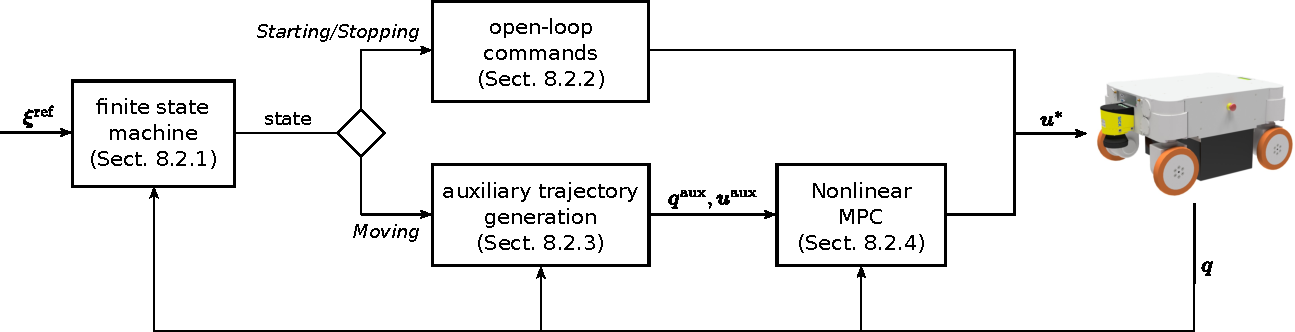
\includegraphics[width=\textwidth]{figures/SWMR/blockscheme.pdf}
    \caption{A block scheme of the proposed framework. A user-defined reference pose trajectory $\bm{\xi}^{\rm ref}$ of the mobile base is used by a FSM to determine when to start and stop the motion of the robot. As soon as a new reference trajectory is available, the state of the FSM becomes \textit{Starting}, and the mobile base is accelerated (using open-loop commands) until all wheel driving velocities are different than zero. When this condition is met, the state of the FSM becomes \textit{Moving}, and the Nonlinear MPC takes full control of the motion of the robot. In this situation, an auxiliary trajectory generation module based on dynamic feedback linearization computes the trajectories $\bm{q}^{\rm aux}$ and $\bm{u}^{\rm aux}$ (using $\bm{\xi}^{\rm ref}$), which are used by the Nonlinear MPC to compute optimal control inputs $\bm{u}^*$. The state of the FSM becomes \textit{Stopping} when $\bm{\xi}^{\rm ref} = \bm{0}$, and the robot is decelerated until it stops.}
    \label{fig:block-scheme}
\end{figure*}

\begin{figure}
    \centering
    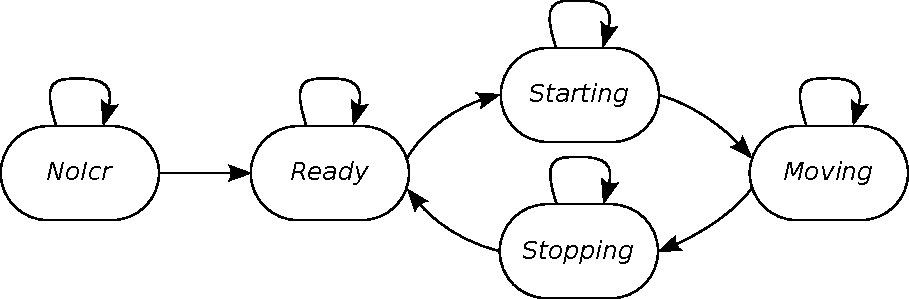
\includegraphics[width=0.7\textwidth]{figures/SWMR/finitestatemachine.pdf}
    \caption{Finite state machine defining the motion of the mobile base.}
    \label{fig:finite-state-machine}
\end{figure}


\subsubsection{ICR constant at infinity}
\label{sec:icr-constant-at-infinity}
in the first case, we assume that the ICR exists and that it is constantly at infinity (i.e., the steering angles are the same for all wheels and $\omega = 0$). Then, the reduced kinematic model of the robot \eqref{eq:reduced-kinematic-model} becomes
\begin{align}
\label{eq:icr-constant-at-infinity-kinematic-model}
\begin{split}
    \dot{x} &= v_{W_1} \cos(\theta + \beta_1) \\
    \dot{y} &= v_{W_1} \sin(\theta + \beta_1), \\
%    \dot{\theta} &= 0 \\
%    \dot{\beta}_1 &= 0,
\end{split}
\end{align}
and the coordinating functions become $\beta_i = h_i(\beta_1) = \beta_1$. In this case, the robot can only move along a line which is parallel to the sagittal axes of the wheels.

\subsubsection{ICR constant not at infinity}
\label{sec:icr-constant-not-at-infinity}
in the second case, we assume an ICR exists and it is at a constant position (different than the position of the steering joints), but not at infinity. Then, the reduced kinematic model of the robot \eqref{eq:reduced-kinematic-model} becomes
\begin{align}
\label{eq:icr-constant-not-at-infinity-kinematic-model}
\begin{split}
    \dot{x} &= \omega R \cos(\theta + \beta_1) + \omega (b_1 \sin\theta + a_1 \cos\theta) \\
    \dot{y} &= \omega R \sin(\theta + \beta_1) + \omega (-b_1 \cos\theta + a_1 \sin\theta) \\
    \dot{\theta} &= \omega, \\
%    \dot{\beta}_1 &= 0,
\end{split}
\end{align}
and the coordinating functions become
\begin{equation*}
    \beta_i = h_i(\beta_1) = \mathrm{arctan}\frac{R \sin\beta_1 + b_i - b_1}{R \cos\beta_1 + a_1 - a_i}.
\end{equation*}
Note that $R$ can be determined from the ICR, which can be computed as the intersection point of the wheel axles. In this case, the robot can only move along the circle centered at the ICR, and radius corresponding to the distance between the position of the robot and the ICR itself. Both the center and the radius are constant, and are determined by the initial configuration of the robot.

\section{Proposed Framework}
\label{sec:proposed-framework}
This section describes in detail the main components of our framework (shown in Fig. \ref{fig:block-scheme}), namely: the finite state machine, responsible for starting and stopping the robot while avoiding kinematic model singularities, the auxiliary trajectory generation module, based on dynamic feedback linearization, which provides trajectories to the NMPC, and the NMPC itself, which computes control inputs for the robot, while satisfying driving and steering velocity constraints on all wheels.

\subsection{Finite state machine}
\label{sec:finite-state-machine}
As mentioned above, since the initial configuration of the robot may be such that the ICR constraint is not satisfied, and since the NMPC must avoid configurations in which coordinating functions \eqref{eq:coordinating-function-post-kinematic-model} are singular (in order to avoid numerical instabilities), we implemented a finite state machine (FSM) to guarantee that the robot is always in a configuration free of singularity.

The FSM, shown in Fig. \ref{fig:finite-state-machine}, consists of five states (\textit{NoICR}, \textit{Ready}, \textit{Starting}, \textit{Moving} and \textit{Stopping}), described -- along with the triggering events -- hereby.
\begin{itemize}
    %\renewcommand{\labelitemi}{$\blacktriangleright$}
    \item[$\blacktriangleright$] \textit{NoICR}. The configuration of the robot is such that the ICR constraint is not satisfied. In this state, the wheels are regulated to a user-defined configuration using a proportional controller.
        \begin{itemize}
            \item[$\bullet$] Once the ICR constraint is satisfied, the state of the FSM becomes \textit{Ready}.
        \end{itemize}
    \item[$\blacktriangleright$] \textit{Ready}. The configuration of the robot is such that the ICR constraint is satisfied and the robot is not moving.
        \begin{itemize}
            \item[$\bullet$] Once a new trajectory is available, the state of the FSM becomes \textit{Starting}.
        \end{itemize}
    \item[$\blacktriangleright$] \textit{Starting}. An open loop controller makes the robot start its motion taking into account the free-of-singularities kinematic models previously presented: either \eqref{eq:icr-constant-at-infinity-kinematic-model} or \eqref{eq:icr-constant-not-at-infinity-kinematic-model} depending on the initial configuration of the robot.
        \begin{itemize}
            \item[$\bullet$] Once all velocities $\dot{\bm{o}}_{S_i}$ become non-zero, the state of the FSM becomes \textit{Moving}.
        \end{itemize}
    \item[$\blacktriangleright$] \textit{Moving}. The robot is moving using the NMPC.
        \begin{itemize}
            \item[$\bullet$] If the trajectory tracking task is about to be be completed, the state of the FSM becomes \textit{Stopping}.
        \end{itemize}
    \item[$\blacktriangleright$] \textit{Stopping}. Similarly to \textit{Starting}, an open loop motion makes the mobile base reduce its speed until it stops.
        \begin{itemize}
            \item[$\bullet$] Once the robot stops its motion, the state of the FSM becomes \textit{Ready}.
        \end{itemize}
\end{itemize}

\subsection{Starting and stopping}
\label{sec:starting-and-stopping}
In this section, we present our free-of-singularity strategy for handling starting and stopping motions. To this end, we first constrain the ICR to be constant, as already explained in Sect.~\ref{sec:icr-constraint-satisfied}, and accelerate (decelerate) the mobile base along the arc of circle defined by the initial position of the robot and the initial ICR, until all velocities $\dot{\bm{o}}_{S_i}$ are different than zero (until the robot stops its motion).

Assuming the ICR is constant at infinity, the system evolves according to~\eqref{eq:icr-constant-at-infinity-kinematic-model}. Considering the driving acceleration~$a_{W_1}$ as control input:
\begin{itemize}
    \item when the state of the FSM is \textit{Starting}, we accelerate the mobile base by choosing $a_{W_1} = a_{W_1}^{\mathrm{init}}$, where $a_{W_1}^{\mathrm{init}}$ is a hyperparameter;
    \item when the state of the FSM is \textit{Stopping}, we decelerate the mobile base by choosing $a_{W_1} = -K_{v_{W_1}}^{\mathrm{stop}} v_{W_1}$, with $K_{v_{W_1}}^{\mathrm{stop}} > 0$.
\end{itemize}

Assuming that the ICR is constant, but not at infinity and not lying on any of the steering joint positions, the system evolves according to~\eqref{eq:icr-constant-not-at-infinity-kinematic-model}.
Considering the angular acceleration $a_{\omega}$ as control input:
\begin{itemize}
    \item when the state of the FSM is \textit{Starting}, we accelerate the mobile base via $a_{\omega} = a_{W_1}^{\mathrm{init}} / R$, which, since $\dot{v}_{W_1}=a_{\omega} R$, is equivalent to accelerate $W_1$ by $a_{W_1}^{\mathrm{init}}$;
    \item when the state of the FSM is \textit{Stopping}, we decelerate the mobile base via $a_{\omega} = -K_{v_{W_1}}^{\mathrm{stop}} v_{W_1} / R$, which is equivalent to decelerate $W_1$ by $-K_{v_{W_1}}^{\mathrm{stop}} v_{W_1}$.
\end{itemize}

\subsection{Auxiliary trajectory generation}
As already mentioned, once velocities $\dot{\bm{o}}_{S_i}$ become non-zero, the state of the FSM becomes \textit{Moving}, and the robot is controlled by the NMPC. In this section, we develop an auxiliary trajectory generation module based on dynamic feedback linearization \cite{Oriolo2002WMRControlDFL}, whose purpose is to compute auxiliary configuration and control input trajectories for the NMPC, given a reference pose trajectory of the mobile base. Note that both auxiliary trajectory generation and the NMPC are only used when the state of the FSM is \textit{Moving}.

Consider the output function $\bm{z}(\bm{q})=\bm{\xi}$ and dynamically extend the robot state~\eqref{eq:reduced-kinematic-model} by adding the following integrators:
\begin{subequations}
    \begin{align*}
        \dot{v}_{W_1} &= a_{W_1} \\
        \dot{\omega} &= a_{\omega},
    \end{align*}
\end{subequations}
so that $\bm{u} = \left[ a_{W_1}, a_{\omega}, v_{\beta_1} \right]^\top $ are the new control inputs. In the following, unless specified otherwise, we denote the robot configuration with dynamic extension as $\bm{q} = (x, y, \theta, \beta_1, \beta_2, \dots, \beta_{n_s}, v_{W_1}, \omega)^\top$. Note that $\bm{q}$ is a non-minimal configuration. The dynamically extended kinematic model is
\begin{equation}
\label{eq:dynamically-extended-kinematic-model}
\begin{split}
    \dot{x} &= v_{W_1} \cos(\theta + \beta_1) + \omega (b_1 \sin\theta + a_1 \cos\theta) \\
    \dot{y} &= v_{W_1} \sin(\theta + \beta_1) + \omega (-b_1 \cos\theta + a_1 \sin\theta) \\
    \dot{\theta} &= \omega \\
    \dot{\beta}_1 &= v_{\beta_1} \\
    \dot{\beta}_i &= \dot{h}_i(\bm{q}, \bm{u}), \quad i = 2, \dots, n_s \\
    \dot{v}_{W_1} &= a_{{W_1}} \\
    \dot{\omega} &= a_{\omega},
\end{split}
\end{equation}
which, in the following, will be denoted as $\dot{\bm{q}} = \bm{f}(\bm{q}, \bm{u})$.

By deriving twice $\bm{z}(\bm{q})$, we obtain
\begin{equation}
\label{eq:zddot}
    \ddot{\bm{z}}(\bm{q})
    =
    \begin{bmatrix}
        \ddot{x} \\ \ddot{y} \\ \ddot{\theta}
    \end{bmatrix}
    =
    \bm{M}(\bm{q}) +
    \bm{H}(\bm{q})
    \begin{bmatrix}
        a_{W_1} \\ a_{\omega} \\ v_{\beta_1}
    \end{bmatrix},
\end{equation}
with $\bm{M}(\bm{q}) \in \mathbb{R}^3$ and $\bm{H}(\bm{q}) \in \mathbb{R}^{3 \times 3}$ defined as
\begin{align*}
    \bm{M}(\bm{q})
    &=
    \begin{bmatrix}
        -\sin(\theta+\beta_1) \omega v_{W_1} + ( b_1 \cos\theta - a_1 \sin\theta) \omega^2 \\
         \cos(\theta+\beta_1) \omega v_{W_1} + (-b_1 \sin\theta + a_1 \cos\theta) \omega^2 \\
        0
    \end{bmatrix}, \\
    \bm{H}(\bm{q})
    &=
    \begin{bmatrix}
        \mathrm{c}(\theta+\beta_1) &  b_1 \mathrm{s}\theta + a_1 \mathrm{c}\theta & -\mathrm{s}(\theta+\beta_1) v_{W_1} \\
        \mathrm{s}(\theta+\beta_1) & -b_1 \mathrm{c}\theta + a_1 \mathrm{s}\theta &  \mathrm{c}(\theta+\beta_1) v_{W_1} \\
        0 & 1 & 0
    \end{bmatrix},
\end{align*}
where $\mathrm{c}(\cdot)$ and $\mathrm{s}(\cdot)$ respectively denote $\cos(\cdot)$ and $\sin(\cdot)$.

By choosing
\begin{equation*}
    \bm{u} = \begin{bmatrix}
        a_{W_1} \\ a_{\omega} \\ v_{\beta_1}
    \end{bmatrix}
    = \bm{H}(\bm{q})^{-1} \left(\bm{a} - \bm{M}(\bm{q})\right),
\end{equation*}
it is possible to transform~\eqref{eq:zddot} into an equivalent chain of integrators
\begin{equation*}
    \ddot{\bm{z}} = \bm{a},
\end{equation*}
which can be easily stabilized. Indeed, exponential regulation of the trajectory tracking error $\bm{e}(t) = \bm{z}^{\mathrm{ref}}(t)-\bm{z}(t)$, can be achieved by taking
\begin{equation*}
    \bm{a} = \ddot{\bm{z}}^{\mathrm{ref}} + \bm{K}_P \bm{e} + \bm{K}_D \dot{\bm{e}}, \quad \bm{K}_P, \bm{K}_D > 0,
\end{equation*}
with $\bm{z}^{\mathrm{ref}}(t)$ twice differentiable and persistent (i.e., $v_{W_1} \ne 0$) reference trajectory. Note that the above decoupling matrix $\bm{H}(\bm{q})$ is singular at $v_{W_1} = 0$. This kind of singularity is structural for mobile robots \cite{Oriolo2002WMRControlDFL}.

Given the reference trajectories $\bm{\xi}^{\mathrm{ref}}, \dot{\bm{\xi}}^{\mathrm{ref}}, \ddot{\bm{\xi}}^{\mathrm{ref}}$, the scheme (Algorithm \ref{alg:AuxiliaryTrajectoryGeneration}) generates, at each timestep $t_k$, the auxiliary configurations $\bm{q}_{j|k}^{\mathrm{aux}}$ ($j = 0, \dots, N$), together with the auxiliary control inputs $\bm{u}_{j|k}^{\mathrm{aux}}$ ($j = 0, \dots, N-1$). These will be used by the NMPC, described in the next section, to compute control inputs $(a_{W_1, k}, a_{\omega, k}, v_{\beta_1, k})^T$ for the mobile base. Note that the function $\mathrm{Sample}$ discretizes a trajectory given over a time interval $[t_k, t_{k} + N \delta_{\mathrm{MPC}}]$, into $N + 1$ elements, with $\delta_{\mathrm{MPC}}$ timestep of the NMPC, and the function $\bm{F}$ integrates the dynamically extended kinematic model \eqref{eq:dynamically-extended-kinematic-model} using fourth-order Runge-Kutta over a timestep $\delta_{\mathrm{MPC}}$, considering coordinating functions \eqref{eq:coordinating-function-post-kinematic-model} for the coordinated steerable wheels $\beta_2, \dots, \beta_{n_s}$.

\begin{algorithm}
\small
\caption{AuxiliaryTrajectoryGeneration}
\label{alg:AuxiliaryTrajectoryGeneration}
\KwIn{$\bm{\xi}^{\mathrm{ref}}, \dot{\bm{\xi}}^{\mathrm{ref}}, \ddot{\bm{\xi}}^{\mathrm{ref}}$}
\KwOut{$\bm{q}_{0|k}^{\mathrm{aux}}, \dots, \bm{q}_{N|k}^{\mathrm{aux}}, \bm{u}_{0|k}^{\mathrm{aux}}, \dots, \bm{u}_{N-1|k}^{\mathrm{aux}}$}
\BlankLine
$\bm{\xi}_{0|k}^{\mathrm{ref}}, \dots, \bm{\xi}_{N|k}^{\mathrm{ref}} \gets \mathrm{Sample}(\bm{\xi}^{\mathrm{ref}})$\;
$\dot{\bm{\xi}}_{0|k}^{\mathrm{ref}}, \dots, \dot{\bm{\xi}}_{N|k}^{\mathrm{ref}} \gets \mathrm{Sample}(\dot{\bm{\xi}}^{\mathrm{ref}})$\;
$\ddot{\bm{\xi}}_{0|k}^{\mathrm{ref}}, \dots, \ddot{\bm{\xi}}_{N|k}^{\mathrm{ref}} \gets \mathrm{Sample}(\ddot{\bm{\xi}}^{\mathrm{ref}})$\;
$\bm{q}_{0|k}^{\mathrm{aux}} \gets \bm{q}_{0|k}^{\mathrm{ref}}$\;
\For{$j \gets 0$ \KwTo $N - 1$}{
    $\bm{a}_{j|k} \gets \ddot{\bm{z}}_{j|k}^{\mathrm{ref}} + \bm{K}_P (\bm{z}_{j|k}^{\mathrm{ref}} - \bm{z}_{j|k}) + \bm{K}_D (\dot{\bm{z}}_{j|k}^{\mathrm{ref}} - \dot{\bm{z}}_{j|k})$\;
    $\bm{u}_{j|k}^{\mathrm{aux}} \gets \bm{H}(\bm{q}_{j|k}^{\mathrm{aux}})^{-1} (\bm{a}_{j|k} - \bm{M}(\bm{q}_{j|k}^{\mathrm{aux}}))$\;
    $\bm{q}_{j+1|k}^{\mathrm{aux}} \gets \bm{F}(\bm{q}_{j+1|k}^{\mathrm{aux}}, \bm{u}_{j|k}^{\mathrm{aux}})$\;
}
\Return{$\bm{q}_{0|k}^{\mathrm{aux}}, \dots, \bm{q}_{N|k}^{\mathrm{aux}}, \bm{u}_{0|k}^{\mathrm{aux}}, \dots, \bm{u}_{N-1|k}^{\mathrm{aux}}$}\;
\end{algorithm}

%\begin{algorithm}
%\small
%\caption{CoordinateWheels}
%\KwIn{$\bm{q}$}
%\KwOut{$\bm{\beta}^{\mathrm{coord}}$}
%\BlankLine
%\For{$i \gets 2$ \KwTo $n_s$}{
%    $\beta_i \gets h_i(\bm{q})$\;
%}
%$\bm{\beta}^{\mathrm{coord}} \gets (\beta_2, \dots, \beta_{n_s})$\;
%\Return $\bm{\beta}^{\mathrm{coord}}$\;
%\end{algorithm}

\subsection{Nonlinear MPC}
\label{sec:model-predictive-control}
The Nonlinear MPC solves, at each control cycle, a finite horizon constrained OCP, taking into account the kinematic model \eqref{eq:reduced-kinematic-model}, wheel velocity and control inputs constraints, singularities of the coordinating functions \eqref{eq:coordinating-function-post-kinematic-model}, and the singularity of the decoupling matrix $\bm{H}(\bm{q})$ in the auxiliary trajectory generation scheme.
In the following, we will denote as $\mathbb{I}_a^b=\{a,\, \dots,\, b\}\subset\mathbb{N}$ the subset of natural numbers containing all naturals from $a$ to $b$.

The OCP can be defined as 
\begin{equation*}
    %\label{eq:ocp-swmr}
    \begin{aligned}
        \min_{\bm{u}(\cdot)} \;\;
            & \; \Phi(\bm{q}(t_k + T_{\mathrm{MPC}})) + \int_{t_k}^{t_k + T_{\mathrm{MPC}}} \mathcal{L}(\bm{q}, \bm{u}) dt \\
            \text{s.t. } & \dot{\bm{q}} = \bm{f}(\bm{q}, \bm{u}) \\
                         & v_{W_1} \ne 0 \\
                         & v_W^- \le v_{W_i} \le v_W^+,\:  \forall i \in \mathbb{I}_2^{n_s} \\
                         %& v_W^- \le v_{W_i}(\bm{q}, \bm{u}) \le v_W^+, \forall i \in \mathbb{I}_2^{n_s} \\
                         & \dot{\bm{o}}_{S_i} \ne \bm{0},\: \forall i \in \mathbb{I}_1^{n_s} \\
                         & a_W^- \le a_{W_1} \le a_W^+ \\
                         & v_{\beta}^- \le v_{\beta_i} \le v_{\beta}^+,\: \forall i \in \mathbb{I}_1^{n_s} \\
                         %& v_{\beta}^- \le \dot{h}_i(\bm{q}, \bm{u}) \le v_{\beta}^+, \forall i \in \mathbb{I}_2^{n_s} \\
                         & \bm{q}(t_k) = \bm{q}_k,
    \end{aligned}
\end{equation*}
with $T_{\mathrm{MPC}}$ duration of the prediction horizon, stage and terminal cost respectively defined as
\begin{align*}
    \mathcal{L}(\bm{q}, \bm{u}) &= \|\bm{q}^{\mathrm{aux}} - \bm{q}\|_{\bm{W_q}}^2 + \|\bm{u}^{\mathrm{aux}} - \bm{u}\|_{\bm{W_u}}^2 \\
    \Phi(\bm{q}) &= \|\bm{q}^{\mathrm{aux}} - \bm{q}\|_{\bm{W_q}}^2,
\end{align*}
$\bm{W_q}, \bm{W_u}$ positive semi-definite weighting matrices, $v_W^-$ and $v_W^+$ min/max wheel driving velocity, $a_W^-$ and $a_W^+$ min/max wheel driving acceleration, $v_{\beta}^-$ and $v_{\beta}^+$  min/max  wheel steering velocity and $\bm{q}_k$ initial configuration.

Note that the velocity constraints are linear for the coordinating wheel (since $v_{W_1}$ and $v_{\beta_1}$ are part of $\bm{q}$) and nonlinear for the coordinated wheels. In particular, because of the assumption of no lateral skidding \eqref{eq:no-lateral-skidding-constraint}, the driving velocity of the coordinated wheels can be computed as
\begin{equation*}
    v_{W_i} = 
    \begin{bmatrix}
        \cos(\theta + \beta_i) \\
        \sin(\theta + \beta_i)
    \end{bmatrix}^\top \dot{\bm{o}}_{W_i}.
\end{equation*}
Since the steering angles of the coordinated wheels are defined as $\beta_i=h_i(v_{W_1}, \omega, \beta_1)$, the steering velocities can simply be computed as their time derivatives.

%\begin{equation}
%        v_{W_i}(\bm{q}, \bm{u}) = \cos(\theta + \beta_i) \dot{x} + \sin(\theta + \beta_i) \dot{y} + (d - a_i \cos\beta_i + b_i \sin\beta_i) \dot{\theta} + d \dot{\beta}_i.
%\end{equation}
As already mentioned, since the coordinating function $h_i$ is singular when $\dot{\bm{o}}_{S_i}=\bm{0}$, it is important to carefully design the control scheme. A simple strategy to make the NMPC free of singularities, is to never let the position of the $i$-th steering joint be at rest. Since the NMPC is activated only when changing the FSM state from \textit{Starting} to \textit{Moving}, it is possible to constrain $\dot{\bm{o}}_{S_i}$ in such a way to never be $\bm{0}$. Indeed, the constraint $\dot{\bm{o}}_{S_i} \ne \bm{0}$, with a proper change of coordinates, can be rewritten as
\begin{equation*}
    \bm{R}(\theta + \beta_i) \dot{\bm{o}}_{S_i} =
    \begin{bmatrix}
        v_{S_i} \\ 0
    \end{bmatrix} \ne \bm{0},
\end{equation*}
with
\begin{equation*}
    v_{S_i} = 
    \begin{bmatrix}
        \cos(\theta + \beta_i) \\
        \sin(\theta + \beta_i)
    \end{bmatrix}^\top \dot{\bm{o}}_{S_i}.
\end{equation*}

Hence, in order to satisfy the above inequality, we need to have $v_{S_i} \ne 0$, which is equivalent to constrain $\mathrm{sgn}(v_{S_i})$ to be constant. Note that, because of the starting motion described in Sect. \ref{sec:starting-and-stopping}, $v_{S_i}$ is either positive or negative when the NMPC is activated. This implies that the constraint will simply be
\begin{equation*}
\begin{cases}
    v_{S_i} > 0, & \text{if $v_{S_i}(t_0)>0$} \\
    v_{S_i} < 0, & \text{otherwise}
\end{cases},
\end{equation*}
with $t_0$ time of activation of the NMPC. A similar reasoning can be done for the constraint $v_{W_1} \ne 0$, which guarantees subsequent calls of the auxiliary trajectory generation module are free of singularities.

We transcribe the above OCP into a nonlinear programming problem (NLP) by using multiple shooting \cite{Bock1984MultipleShooting}. The resulting NLP is the following:
\begin{equation*}
    \begin{aligned}
        \min_{\bm{Q}_k, \bm{U}_k} \;
            & \Phi(\bm{q}_{N|k}) + \sum_{j=0}^{N-1} \mathcal{L}(\bm{q}_{j|k}, \bm{u}_{j|k}) \\
            \text{s.t. } & \bm{q}_{j+1|k} = \bm{F}(\bm{q}_{j|k}, \bm{u}_{j|k}),\: \forall j \in \mathbb{I}_0^{N-1} \\
                         & \mathrm{sgn}(v_{W_1,j|k}) = \mathrm{sgn}(v_{W_1}(t_0)),\: \forall j \in \mathbb{I}_0^N \\
                         & v_W^- \le v_{W_{i,j|k}}(\cdot) \le v_W^+,\: \forall i \in \mathbb{I}_2^{n_s}, \forall j \in \mathbb{I}_0^{N-1} \\
                         & \mathrm{sgn}(v_{S_{1,j|k}}(\cdot)) = \mathrm{sgn}(v_{S_1}(t_0)),\: \forall j \in \mathbb{I}_0^N \\
                         & \mathrm{sgn}(v_{S_{i,j|k}}(\cdot)) = \mathrm{sgn}(v_{S_i}(t_0)),\: \forall i \in \mathbb{I}_2^{n_s}, \forall j \in \mathbb{I}_0^{N-1} \\
                         & a_W^- \le a_{W_1,j|k} \le a_W^+,\: \forall j \in \mathbb{I}_0^{N-1} \\
                         & v_{\beta}^- \le v_{\beta_1,j|k} \le v_{\beta}^+,\: \forall j \in \mathbb{I}_0^{N-1} \\
                         & v_{\beta}^- \le v_{\beta_i,j|k}(\cdot) \le v_{\beta}^+,\: \forall i \in \mathbb{I}_2^{n_s}, \forall j \in \mathbb{I}_0^{N-1} \\
                         & \bm{q}_{0|k} = \bm{q}_k,
    \end{aligned}
\end{equation*}
with
\begin{align*}
\bm{Q}_k &= (\bm{q}_{0|k}^\top, \bm{q}_{1|k}^\top, \dots, \bm{q}_{N|k}^\top)^\top \\
\bm{U}_k &= (\bm{u}_{0|k}^\top, \bm{u}_{1|k}^\top, \dots, \bm{u}_{N-1|k}^\top)^\top
\end{align*}
collecting the decision variable of the NMPC at $t_k$, $T_{\mathrm{MPC}}=N\delta_{\mathrm{MPC}}$, $\delta_{\mathrm{MPC}}$ timestep of the NMPC, and the cost function evaluated using $\bm{q}_{j|k}^{\mathrm{aux}}$ ($j = 0, \dots, N$) and $\bm{u}_{j|k}^{\mathrm{aux}}$ ($j = 0, \dots, N - 1$), computed by the auxiliary trajectory generation module. Notice that, within the constraints of the NLP, we used $(\cdot)$ to denote the use of nonlinear functions.

Once the NLP is solved, the control sample $\bm{u}_{0|k}$ is extracted from $\bm{U}_k$, and it is used to compute the driving and steering velocities which realize it, that are sent to the robot.

% \subsection{NMPC}
% The above optimal control problem \eqref{eq:ocp-swmr} can be transcribed to a nonlinear programming problem by properly discretizing the cost function and the constraints.

% Discretizing $\bm{\dot{q}} = \bm{v}$:
% \begin{equation}
%     \bm{q}_{k+1} = q_k + \delta \bm{v}_k
% \end{equation}
% with $\delta = t_{k+1} - t_{k}$.

% Discretizing no lateral skidding constraint \eqref{eq:no-lateral-skidding-constraint}, when $t \in [t_k, t_{k+1}]$:
% \begin{equation}
%     \label{eq:no-lateral-skidding-constraint-discretized}
%     g_{i,k}^{\rm skid}(\bm{q}_k, \bm{v}_k) = -\sin(\theta_k + \beta_{i,k}) \dot{x}_k +
%     \cos(\theta_k + \beta_{i,k}) \dot{y}_k +
%     (b_i \cos(\beta_{i,k}) + a_i \sin(\beta_{i,k})) \dot{\theta}_k = 0
% \end{equation}

% Discretizing rolling with no slipping constraint \eqref{eq:rolling-with-no-slipping-constraint}, when $t \in [t_k, t_{k+1}]$:
% \begin{equation}
%     \begin{split}
%         \label{eq:rolling-with-no-slipping-constraint-discretized}
%         g_{i,k}^{\rm slip}(\bm{q}_k, \bm{v}_k) = \cos(\theta_k + \beta_{i,k}) \dot{x}_k +
%         \sin(\theta_k + \beta_{i,k}) \dot{y}_k + \\
%         (d  - a_i \cos(\beta_{i,k}) + b_i \sin(\beta_{i,k})) \dot{\theta}_k +
%         d \dot{\beta}_{i,k}
%         -r_w \dot{\phi}_{i,k} = 0
%     \end{split}
% \end{equation}

% It is possible to define a NMPC:
% \begin{equation}
%     \label{eq:nmpc}
%     \begin{aligned}
%         \min_{\bm{q}_k, \bm{v}_k} \;
%             & L(\bm{q}_k, \bm{v}_k) \\
%             \text{s.t. } & \bm{q}_{k+1} = q_k + \delta \bm{v}_k \\
%                          & \text{no lateral skidding constraint \eqref{eq:no-lateral-skidding-constraint-discretized}} \\
%                          & \text{rolling with no slipping constraint \eqref{eq:rolling-with-no-slipping-constraint-discretized}}
%     \end{aligned}
% \end{equation}

% \subsection{Real-time iteration}
% The NMPC \eqref{eq:nmpc} can be  efficiently solved by  using real-time iteration \cite{Gros2020Fromlineartononlinear}.

% Linearize no lateral skidding constraint \eqref{eq:no-lateral-skidding-constraint-discretized} around reference trajectory:
% \begin{equation}
%     g_{i,k}^{\rm skid}(\bm{q}_k^{\rm ref}, \bm{v}_k^{\rm ref}) +
%     \left. \frac{\partial g_{i,k}^{\rm skid}}{\partial \bm{q}} \right|_{\bm{q}_k^{\rm ref}, \bm{v}_k^{\rm ref}} (\bm{q}_k^{\rm ref} - \bm{q}_k) +
%     \left. \frac{\partial g_{i,k}^{\rm skid}}{\partial \bm{v}} \right|_{\bm{q}_k^{\rm ref}, \bm{v}_k^{\rm ref}} (\bm{v}_k^{\rm ref} - \bm{v}_k) = 0
% \end{equation}

% Linearize rolling with no slipping constraint \eqref{eq:rolling-with-no-slipping-constraint-discretized} around reference trajectory:
% \begin{equation}
%     g_{i,k}^{\rm slip}(\bm{q}_k^{\rm ref}, \bm{v}_k^{\rm ref}) +
%     \left. \frac{\partial g_{i,k}^{\rm slip}}{\partial \bm{q}} \right|_{\bm{q}_k^{\rm ref}, \bm{v}_k^{\rm ref}} (\bm{q}_k^{\rm ref} - \bm{q}_k) +
%     \left. \frac{\partial g_{i,k}^{\rm slip}}{\partial \bm{v}} \right|_{\bm{q}_k^{\rm ref}, \bm{v}_k^{\rm ref}} (\bm{v}_k^{\rm ref} - \bm{v}_k) = 0
% \end{equation}

%Considering all the above kinematic constraints in Pfaffian form and rewriting them in matrix form $\bm{A}^\top(\bm{q}) \bm{\dot{q}} = 0$:
%\begin{equation}
%    \begin{bmatrix}
%        -\sin(\theta + \beta_1) &
%        \cos(\theta + \beta_1) &
%        b_1 \cos(\beta_1) + a_1 \sin(\beta_1) &
%        0 & 0 & 0 & 0 & 0 & 0 & 0 & 0 \\
%        -\sin(\theta + \beta_2) &
%        \cos(\theta + \beta_2) &
%        b_2 \cos(\beta_2) + a_2 \sin(\beta_2) &
%        0 & 0 & 0 & 0 & 0 & 0 & 0 & 0 \\
%        -\sin(\theta + \beta_3) &
%        \cos(\theta + \beta_3) &
%        b_3 \cos(\beta_3) + a_3 \sin(\beta_3) &
%        0 & 0 & 0 & 0 & 0 & 0 & 0 & 0 \\
%        -\sin(\theta + \beta_4) &
%        \cos(\theta + \beta_4) &
%        b_4 \cos(\beta_4) + a_4 \sin(\beta_4) &
%        0 & 0 & 0 & 0 & 0 & 0 & 0 & 0 \\
%        \cos(\theta + \beta_1) &
%        \sin(\theta + \beta_1) &
%        d  - a_1 \cos(\beta_1) + b_1 \sin(\beta_1) &
%        d & -r_w & 0 & 0 & 0 & 0 & 0 & 0 \\
%        \cos(\theta + \beta_2) &
%        \sin(\theta + \beta_2) &
%        d  - a_2 \cos(\beta_2) + b_2 \sin(\beta_2) &
%        0 & 0 & d & -r_w & 0 & 0 & 0 & 0 \\
%        \cos(\theta + \beta_3) &
%        \sin(\theta + \beta_3) &
%        d  - a_3 \cos(\beta_3) + b_3 \sin(\beta_3) &
%        0 & 0 & 0 & 0 & d & -r_w & 0 & 0 \\
%        \cos(\theta + \beta_4) &
%        \sin(\theta + \beta_4) &
%        d  - a_4 \cos(\beta_4) + b_4 \sin(\beta_4) &
%        0 & 0 & 0 & 0 & 0 & 0 & d & -r_w \\
%    \end{bmatrix}
%    \bm{\dot{q}} = 0
%\end{equation}

%Let $\bm{A}_1^\top(\bm{q})$ be the left submatrix of $\bm{A}^\top(\bm{q})$ of size $8 \times 3$ and $\bm{A}_2^\top(\bm{q})$ be the right submatrix of $\bm{A}^\top(\bm{q})$ of size $8 \times 8$, then:
%\begin{equation}
%    \bm{A}_1^\top(\bm{q})
%    \begin{bmatrix}
%        \dot{x} \\
%        \dot{y} \\
%        \dot{\theta}
%    \end{bmatrix}
%    =
%    -\bm{A}_2^\top(\bm{q})
%    \begin{bmatrix}
%        \dot{\beta}_1 \\
%        \dot{\phi}_1 \\
%        \dot{\beta}_2 \\
%        \dot{\phi}_2 \\
%        \dot{\beta}_3 \\
%        \dot{\phi}_3 \\
%        \dot{\beta}_4 \\
%        \dot{\phi}_4
%    \end{bmatrix}
%\end{equation}
%which can be rewritten as:
%\begin{equation}
%    \bm{\dot{\xi}} =
%    (\bm{A}_1^\top(\bm{q}))^+ \begin{bmatrix}
%        \bm{0}_4 \\
%         r_w \bm{\dot{\phi}} - d \bm{\dot{\beta}}
%    \end{bmatrix}
%\end{equation}
%with $\bm{\dot{\xi}} = [\dot{x}, \dot{y}, \dot{\theta}]^\top$, $\bm{\dot{\phi}} = [\dot{\phi}_1, \dot{\phi}_2, \dot{\phi}_3, \dot{\phi}_4]^\top$ and $\bm{\dot{\beta}} = [\dot{\beta}_1, \dot{\beta}_2, \dot{\beta}_3, \dot{\beta}_4]^\top$. {\color{red} Why odometry model in Sorour has lateral skidding constraints missing (i.e., the $\bm{0}_4$ part)?}

%\section{Model Predictive Control}
%Idea: MPC as QP using equation of motion found in section odometry model, linear constraints on inputs (mimimum and maximum velocity), cost function on $\bm{\xi}$ and $\bm{\dot{\xi}}$. Odometry model needs to be linearized.

%\subsection{Wheel coordination}
%Since the low-level controller of the platform requires the steering velocities $\dot{\beta}_i$ and the angular velocities of the wheels $\dot{\phi}_i=v_{W_i}/r_w$ (with $r_w$ radius of the wheels), it is important to compute this quantities taking into account wheel coordination and wheel slipping.

%To avoid slipping of the wheel, the projection of the velocity of the center of the wheel along the sagittal axis of the wheel must be equal to the velocity of the wheel itself:
%\begin{equation}
%    v_{W_i} =
%    \begin{bmatrix}
%        \cos(\theta + \beta_i) \\
%        \sin(\theta + \beta_i)
%    \end{bmatrix}^\top \dot{\bm{o}}_{W_i} = r_w \dot{\phi}_i,
%\end{equation}
%hence $\dot{\phi}_i = v_{W_i}/r_w$.

\section{Experiments}
\label{sec:simulations-and-experiments}
The proposed framework has been implemented in Python, using the acados library \cite{Verschueren2021acados} to solve the aforementioned NLP with the real-time iteration scheme \cite{Gros2020Fromlineartononlinear}. The mobile base used is the Neobotix MPO-700, which is equipped with $n_s=4$ steerable wheels. The scheme runs at 75 Hz on an Intel Core i5-10210U (1.6 GHz, 8 cores) with Ubuntu 20.04 LTS.

We validate our implementation on a series of trajectory tracking experiments with increasing complexity. In particular, we define a reference pose trajectory using a geometric path $\bm{\xi}^{\mathrm{ref}}(s)$ and a timing law $s(t)$. All timing laws $s(t)$ used below are 5-th order polynomials such that:
\begin{equation*}
s(t_0) = \dot{s}(t_0) = \dot{s}(t_f) = \ddot{s}(t_0) = \ddot{s}(t_f)=0, s(t_f)=1,
\end{equation*}
with $s \in [0, 1]$, and with $t_0$ and $t_f$ respectively initial and final time of the reference trajectory. This guarantees that all trajectories are defined with initial and final velocity set to zero, and with initial and final acceleration set to zero. In the following, we will use $t_0 = 0.0$ [s], and we will assume that the initial position of the robot is $x_0 = 0.0$~[m], $y_0 = 0.0$~[m].

The hyperparameters used are listed in Table \ref{tab:hyperparameters}. Video clips of the described experiments are included in the accompanying video. %Video clips of the described experiments are available at YOUTUBE LINK HERE.

\begin{table}
\centering
\caption{Hyperparameters used in all our experiments.}
\begin{tabular}{ |c|c| } 
    \hline
    Symbol & Value \\
    \hline
    $\bm{a}$ & $(-0.19, 0.19, 0.19, -0.19)$ [m] \\
    $\bm{b}$ & $(0.24, 0.24, -0.24, -0.24)$ [m] \\
    $d$ & 0.045 [m] \\
    $a_{W_1}^{\mathrm{init}}$ & $0.1$ [m/s$^2$] \\ 
    $K_{v_{W_1}}^{\mathrm{stop}}$ & $1.0$ \\ 
    $\bm{K}_P$ & $\mathrm{diag}(4.0, 4.0, 2.0)$ \\ 
    $\bm{K}_D$ & $\mathrm{diag}(2.0, 2.0, 1.0)$ \\ 
    $N$ & 5 \\
    $\delta_{\mathrm{MPC}}$ & 0.1 [s] \\
    $\bm{W_q}$ & $\bm{I}_9$ \\ 
    $\bm{W_u}$ & $\bm{I}_3$ \\
    $v_W^-$ & -0.9 [m/s] \\
    $v_W^+$ & 0.9 [m/s] \\
    $a_W^-$ & $-0.5$ [m/s$^2$] \\ 
    $a_W^+$ & $0.5$ [m/s$^2$] \\ 
    $v_{\beta}^-$ & $-2.0$ [rad/s] \\ 
    $v_{\beta}^+$ & $2.0$ [rad/s] \\ 
    \hline
\end{tabular}
\label{tab:hyperparameters}
\end{table}

\subsection{Straight line motions}
The \textit{forward motion} trajectory, consists in the robot moving along a straight line, without changing its orientation. It is defined by
\begin{equation*}
\renewcommand{\arraystretch}{1.3}
\begin{array}{c}
    \begin{aligned}
        x^{\mathrm{ref}}(s) &= x_0 + s (x_f - x_0) \\
        y^{\mathrm{ref}}(s) &= y_0 + s (y_f - y_0) \\
        \theta^{\mathrm{ref}}(s) &= \theta_0
    \end{aligned}  \\
    \begin{aligned}
        x_f &= x_0 + v^{\mathrm{ref}} \cos(\theta^{\mathrm{dir}}) (t_f - t_0) \\
        y_f &= y_0 + v^{\mathrm{ref}} \sin(\theta^{\mathrm{dir}}) (t_f - t_0),
     \end{aligned}
\end{array}
\end{equation*}
$\theta_{\mathrm{dir}}=\theta_0$ and $v^{\mathrm{ref}}>0$. The initial orientation of the robot is $\theta_0=0.0$ [rad], and the initial configuration of the steering angles is given by$\beta_{1,0}=\beta_{2,0}=\beta_{3,0}=\beta_{4,0}=0.0$ [rad]. Moreover, $t_f = 25.0$ [s] and $v^{\mathrm{ref}}=0.2$ [m/s].%Figure \ref{fig:experiments:forward:snapshots} shows a sequence of snapshots of the mobile base moving while tracking the considered trajectory. Figure \ref{fig:simulations:forward:inputs-and-errors} show the control inputs computed by the NMPC and the trajectory tracking error. Figure \ref{fig:simulations:forward:wheel-velocities} shows the corresponding driving and steering velocities.
%\begin{figure*}
%    \centering
%    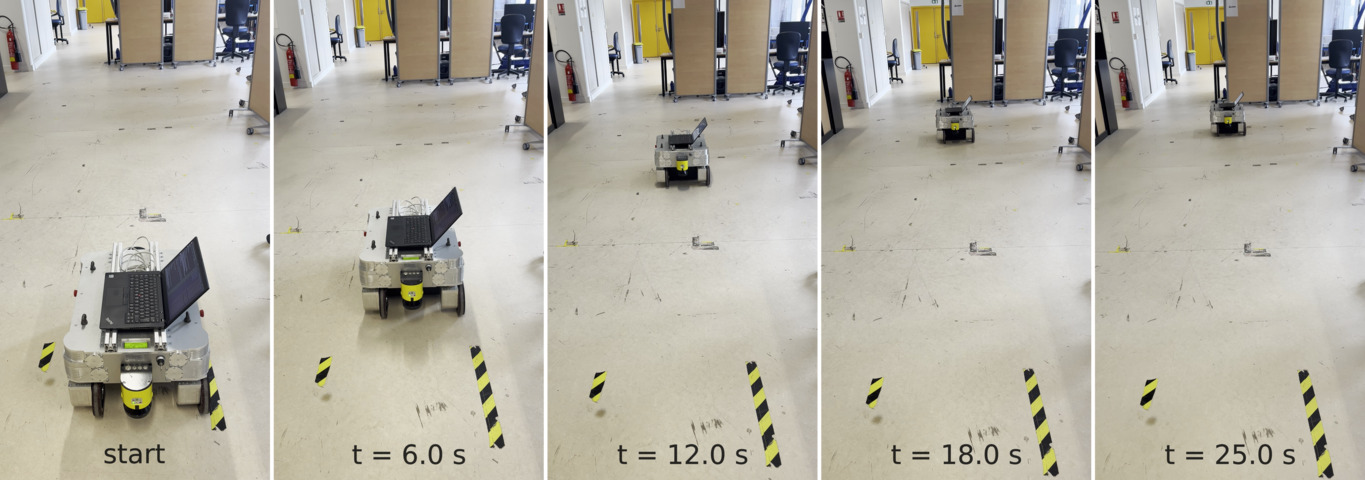
\includegraphics[width=\textwidth]{figures/SWMR/simulations/forward/snapshots.jpeg}
%    \caption{Snapshots of the mobile base tracking a \textit{forward motion} trajectory.}
%    \label{fig:experiments:forward:snapshots}
%\end{figure*}
%\begin{figure*}
%    \centering
%    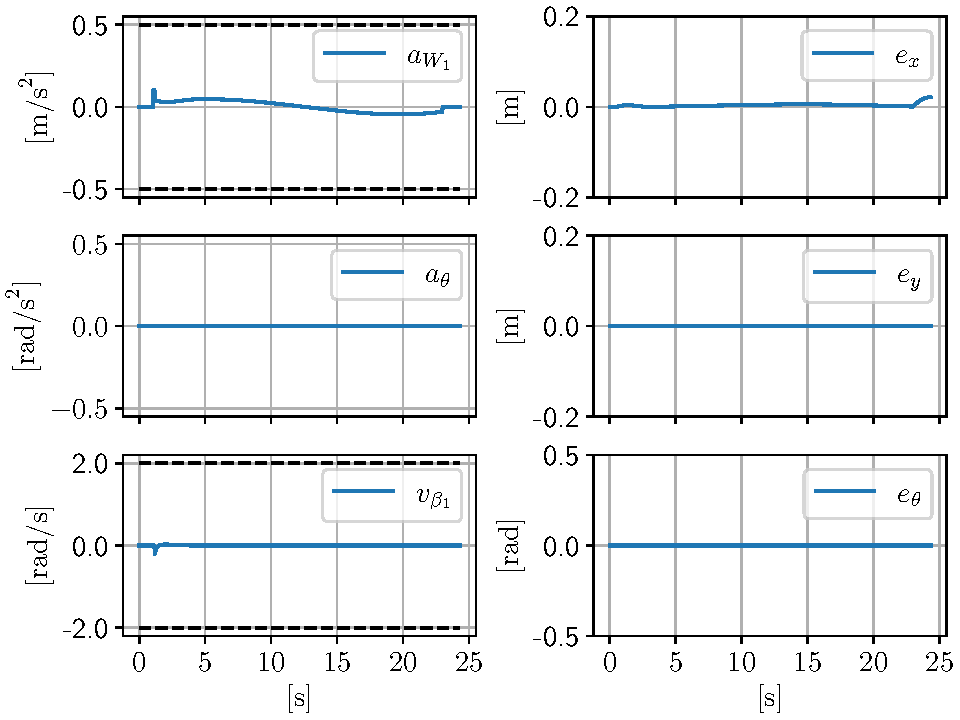
\includegraphics[width=0.8\textwidth]{figures/SWMR/simulations/forward/inputs_and_errors.pdf}
%    \caption{Control inputs and trajectory tracking errors for the \textit{forward motion} trajectory.}
%    \label{fig:simulations:forward:inputs-and-errors}
%\end{figure*}
%\begin{figure*}
%    \centering
%    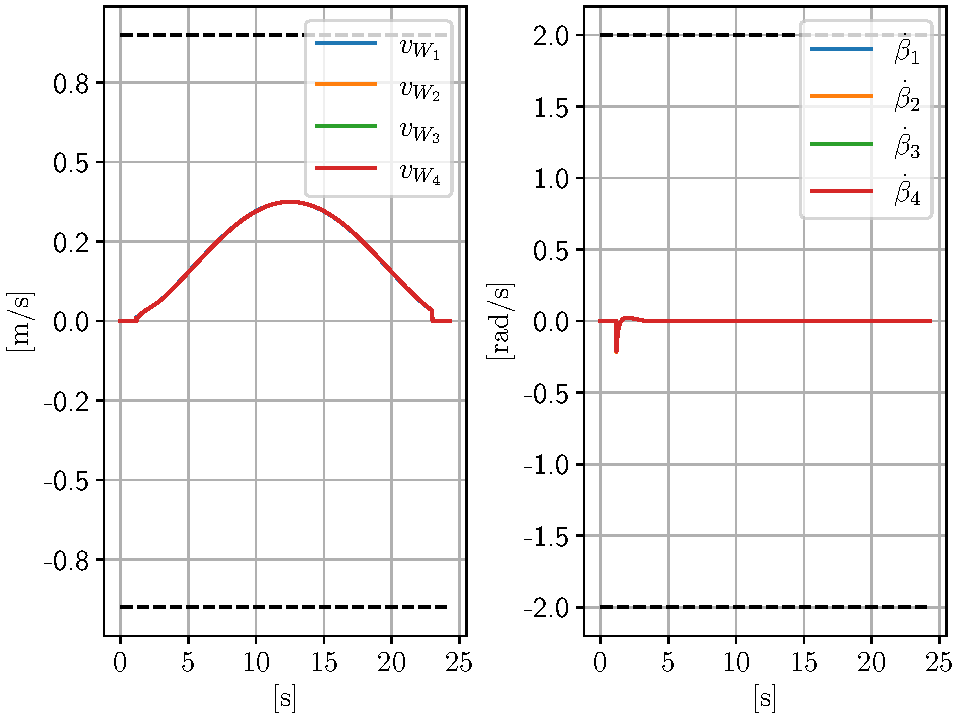
\includegraphics[width=0.8\textwidth]{figures/SWMR/simulations/forward/wheels_velocities.pdf}
%    \caption{Driving and steering velocities of the four wheels for the \textit{forward motion} trajectory.}
%    \label{fig:simulations:forward:wheel-velocities}
%\end{figure*}

The \textit{backward motion} trajectory is defined similarly to the \textit{forward motion} trajectory, with the difference that $v^{\mathrm{ref}}<0$. The initial orientation of the robot is $\theta_0=0.0$ [rad]. Moreover, $\beta_{1,0}=\beta_{2,0}=\beta_{3,0}=\beta_{4,0}=\pi$ [rad], $t_f = 25.0$ [s] and $v^{\mathrm{ref}}=0.2$ [m/s]. %Figure \ref{fig:experiments:backward:snapshots} shows a sequence of snapshots of the mobile base moving while tracking the considered trajectory. Figure \ref{fig:simulations:backward:inputs-and-errors} show the control inputs computed by the NMPC and the trajectory tracking error. Figure \ref{fig:simulations:backward:wheel-velocities} shows the corresponding driving and steering velocities.
%\begin{figure*}
%    \centering
%    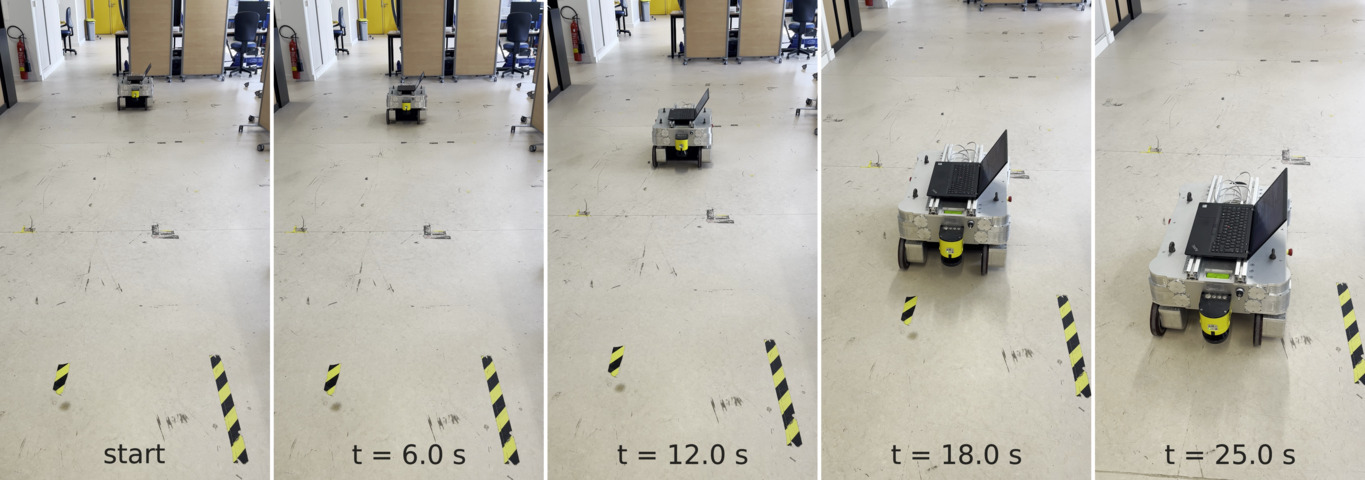
\includegraphics[width=\textwidth]{figures/SWMR/simulations/backward/snapshots.jpeg}
%    \caption{Snapshots of the mobile base tracking a \textit{backward motion} trajectory.}
%    \label{fig:experiments:backward:snapshots}
%\end{figure*}
%\begin{figure*}
%    \centering
%    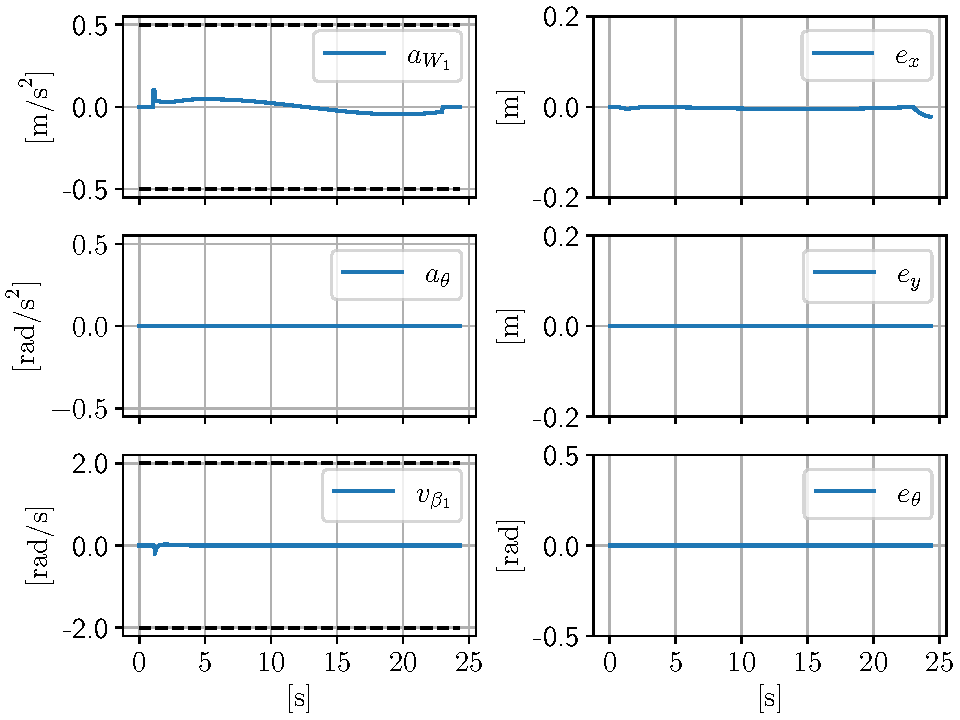
\includegraphics[width=0.8\textwidth]{figures/SWMR/simulations/backward/inputs_and_errors.pdf}
%    \caption{Control inputs and trajectory tracking errors for the \textit{backward motion} trajectory.}
%    \label{fig:simulations:backward:inputs-and-errors}
%\end{figure*}
%\begin{figure*}
%    \centering
%    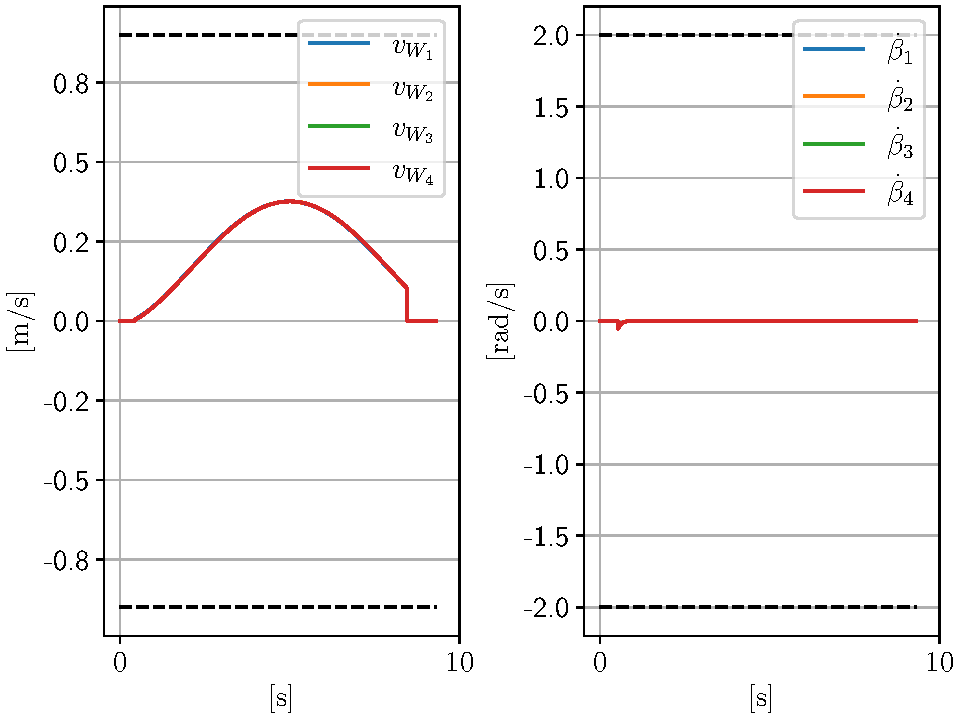
\includegraphics[width=0.8\textwidth]{figures/SWMR/simulations/backward/wheels_velocities.pdf}
%    \caption{Driving and steering velocities of the four wheels for the \textit{backward motion} trajectory.}
%    \label{fig:simulations:backward:wheel-velocities}
%\end{figure*}

The \textit{diagonal motion} trajectory is defined similarly to the \textit{forward motion} trajectory, but with $\theta^{\mathrm{dir}} \ne \theta_0$. The initial orientation of the robot is $\theta_0=\pi/4$ [rad]. Moreover, $\beta_{1,0}=\beta_{2,0}=\beta_{3,0}=\beta_{4,0}=-\pi/4$ [rad], $t_f = 25.0$ [s] and $v^{\mathrm{ref}}=0.2$ [m/s]. %Figure \ref{fig:experiments:diagonal:snapshots} shows a sequence of snapshots of the mobile base moving while tracking the considered trajectory. Figure \ref{fig:simulations:diagonal:inputs-and-errors} show the control inputs computed by the NMPC and the trajectory tracking error. Figure \ref{fig:simulations:diagonal:wheel-velocities} shows the corresponding driving and steering velocities.
%\begin{figure*}
%    \centering
%    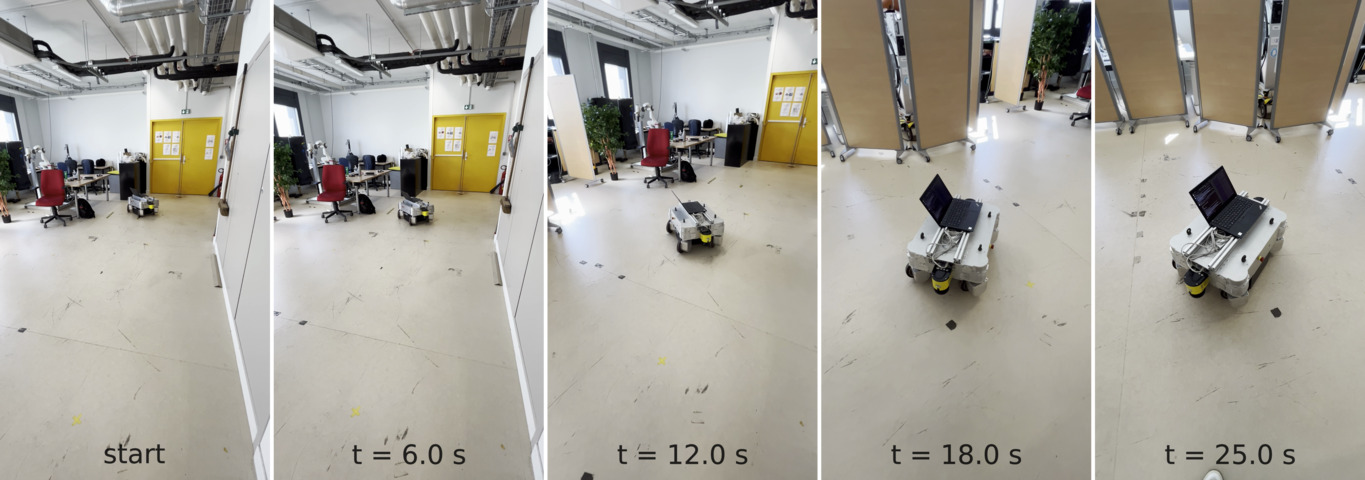
\includegraphics[width=\textwidth]{figures/SWMR/simulations/diagonal/snapshots.jpeg}
%    \caption{Snapshots of the mobile base tracking a \textit{diagonal motion} trajectory.}
%    \label{fig:experiments:diagonal:snapshots}
%\end{figure*}
%\begin{figure*}
%    \centering
%    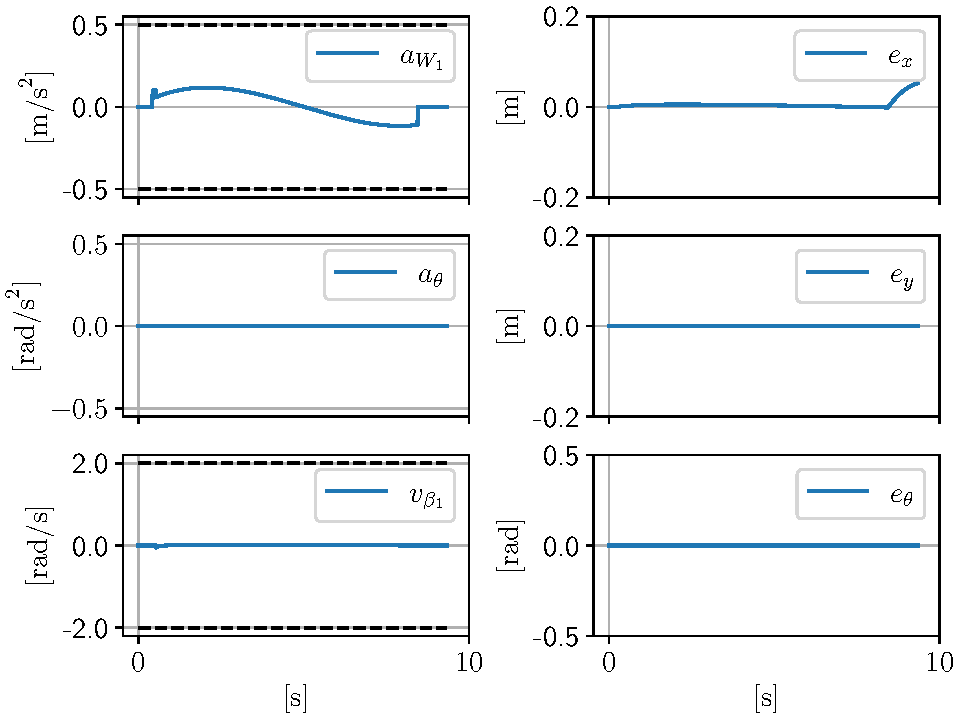
\includegraphics[width=0.8\textwidth]{figures/SWMR/simulations/diagonal/inputs_and_errors.pdf}
%    \caption{Control inputs and trajectory tracking errors for the \textit{diagonal motion} trajectory.}
%    \label{fig:simulations:diagonal:inputs-and-errors}
%\end{figure*}
%\begin{figure*}
%    \centering
%    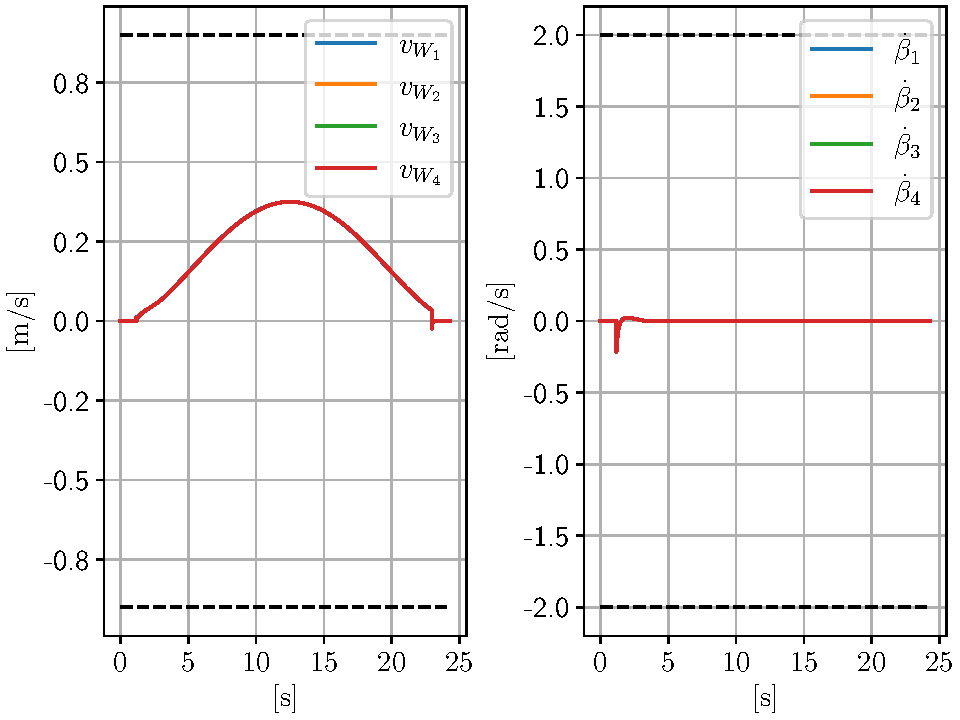
\includegraphics[width=0.8\textwidth]{figures/SWMR/simulations/diagonal/wheels_velocities.pdf}
%    \caption{Driving and steering velocities of the four wheels for the \textit{diagonal motion} trajectory.}
%    \label{fig:simulations:diagonal:wheel-velocities}
%\end{figure*}

In all these experiments (\textit{forward}, \textit{backward} and \textit{diagonal motion}), the reference position of the robot is the same. The reference orientation, on the other hand, is different. Note that the robot is able to track diagonal trajectories because of the steerable wheels, which allow the mobile base behave as an omnidirectional robot.

\subsection{Circular motions}
In this section, we consider tasks in which the robot is required to follow a circle with center $(x_C, y_C)$ and radius $R > 0$. The reference position, which is in common among all circular trajectories (defined below), is given by
\begin{subequations}
    \begin{align*}
        x^{\mathrm{ref}}(s) &= x_C + R \cos(\phi + 2 \pi s) \\
        y^{\mathrm{ref}}(s) &= y_C + R \sin(\phi + 2 \pi s).
    \end{align*} 
\end{subequations}

In the \textit{circle with constant orientation} trajectory, the reference orientation is defined by
\begin{subequations}
\begin{align*}
    \theta^{\mathrm{ref}}(t) &= \theta_0,
\end{align*}
\end{subequations}
with $\theta_0=\pi$ [rad]. The initial configuration of the steering angles are given by$\beta_{1,0}=\beta_{2,0}=\beta_{3,0}=\beta_{4,0}=0.0$ [rad]. Moreover, $R=0.5$ [m], $\phi=\pi/2$ [rad], and $t_f=15.7$~[s].

Similarly to the \textit{diagonal motion}, the robot is able to track a circle while keeping its orientation constant because of the steerable wheels. This kind of motion, indeed, would not be possible with a differential drive robot.
%Figure \ref{fig:experiments:circle-with-constant-orientation:snapshots} shows a sequence of snapshots of the mobile base moving while tracking the considered trajectory. Figure \ref{fig:simulations:circle-with-constant-orientation:inputs-and-errors} show the control inputs computed by the NMPC and the trajectory tracking error. Figure \ref{fig:simulations:circle-with-constant-orientation:wheel-velocities} shows the corresponding driving and steering velocities.
%\begin{figure*}
%    \centering
%    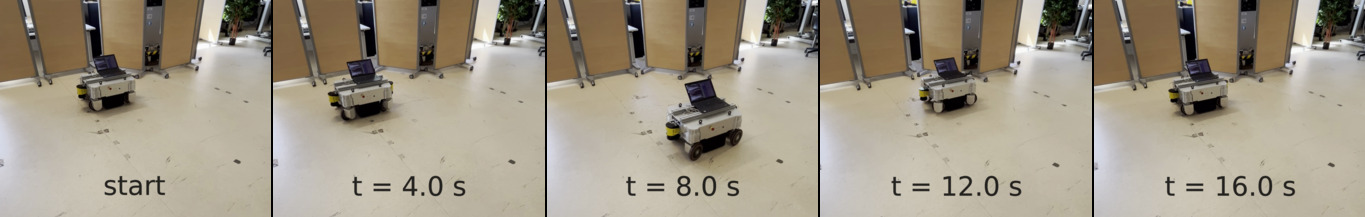
\includegraphics[width=\textwidth]{figures/SWMR/simulations/circular_with_constant_orientation/snapshots.jpeg}
%    \caption{Snapshots of the mobile base tracking a \textit{circle with constant orientation}.}
%    \label{fig:experiments:circle-with-constant-orientation:snapshots}
%\end{figure*}
%\begin{figure*}
%    \centering
%    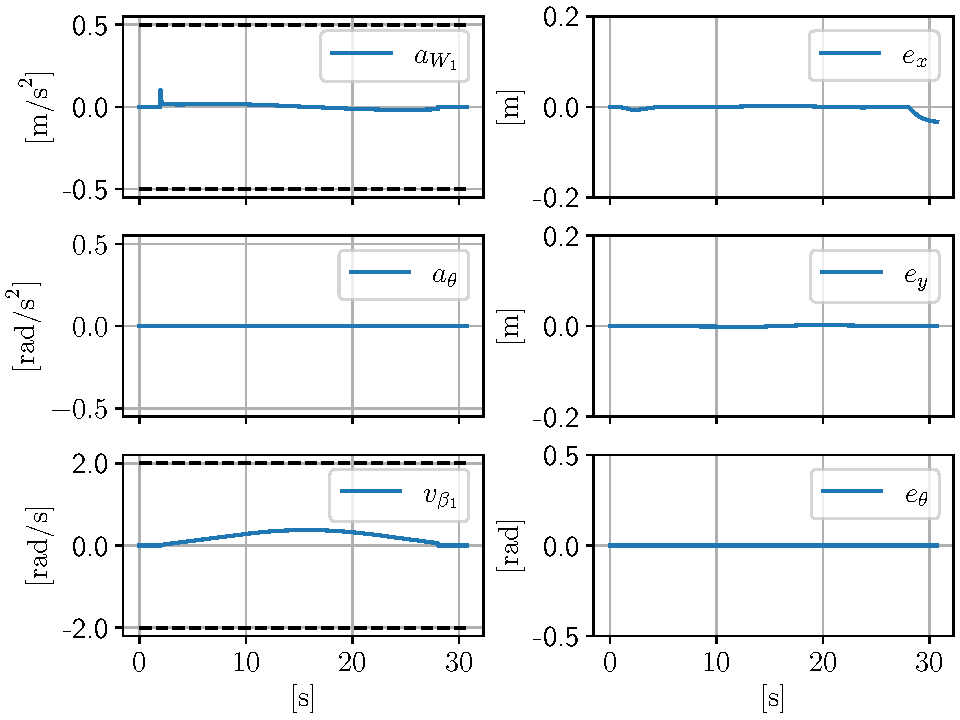
\includegraphics[width=0.8\textwidth]{figures/SWMR/simulations/circular_with_constant_orientation/inputs_and_errors.pdf}
%    \caption{Control inputs and trajectory tracking errors for the \textit{circle with constant orientation} trajectory.}
%    \label{fig:simulations:circle-with-constant-orientation:inputs-and-errors}
%\end{figure*}
%\begin{figure*}
%    \centering
%    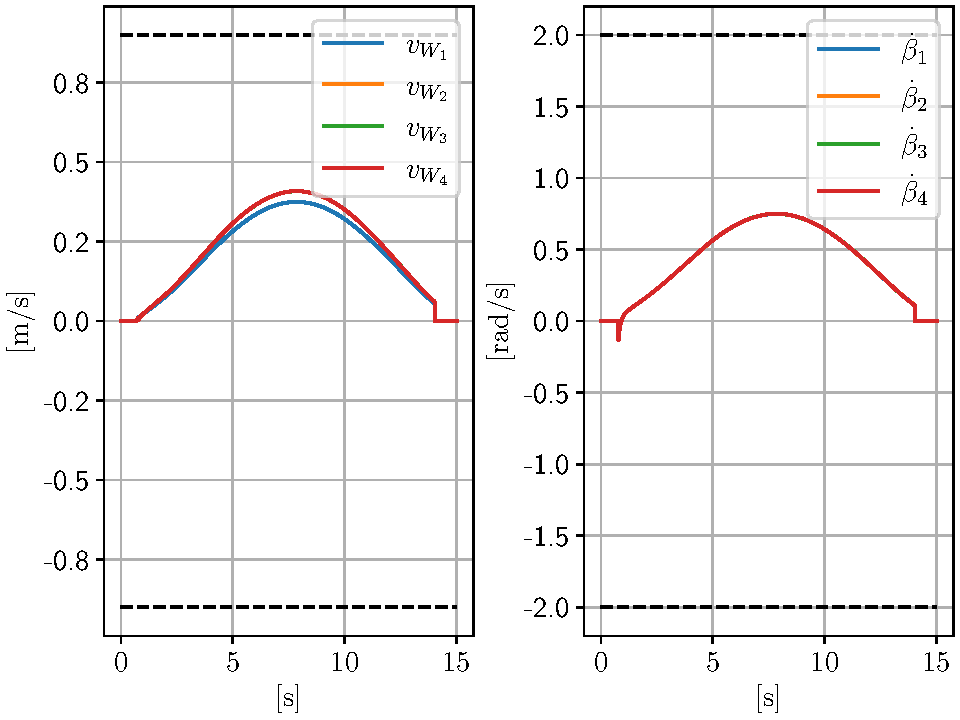
\includegraphics[width=0.8\textwidth]{figures/SWMR/simulations/circular_with_constant_orientation/wheels_velocities.pdf}
%    \caption{Driving and steering velocities of the four wheels for the \textit{circle with constant orientation} trajectory.}
%    \label{fig:simulations:circle-with-constant-orientation:wheel-velocities}
%\end{figure*}

In the \textit{circle with tangent orientation} trajectory, the reference orientation is defined by
\begin{equation}
    \theta^{\mathrm{ref}}(s) = \mathrm{atan2}\left(\frac{\partial y^{\mathrm{ref}}(s)}{\partial s}, \frac{\partial x^{\mathrm{ref}}(s)}{\partial s}\right).
    \label{eq:reference-tangent-orientation}
\end{equation}
Here, $\theta_0=\pi$ [rad], $\beta_{1,0}=\beta_{2,0}=\beta_{3,0}=\beta_{4,0}=0.0$ [rad]. Moreover, $R=0.5$ [m], $\phi=\pi/2$ [rad], and $t_f=15.7$~[s].
Figure \ref{fig:experiments:circle-with-tangent-orientation:snapshots} shows a sequence of snapshots of the robot moving while tracking this trajectory. Here, it is possible to notice how the mobile base changes its orientation according to the previously defined circle, ending up in its initial pose at the end of the motion. Figure \ref{fig:simulations:circle-with-tangent-orientation:inputs-and-errors} show the control inputs computed by the NMPC, together with the trajectory tracking error. Figure \ref{fig:simulations:circle-with-tangent-orientation:wheel-velocities} shows the corresponding driving and steering velocities. In these last two plots it is possible to appreciate the behavior of the NMPC. The trajectory tracking error is always close to zero, and the control inputs, together with steering and driving velocities of the wheels, are always within their boundaries.
\begin{figure*}
    \centering
    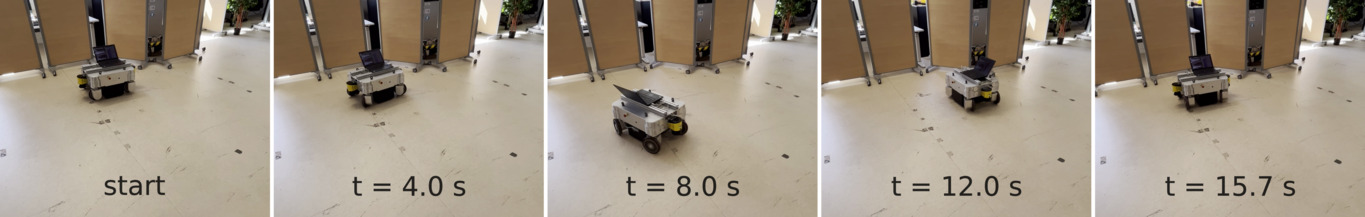
\includegraphics[width=\textwidth]{figures/SWMR/simulations/circular_with_tangent_orientation/snapshots.jpeg}
    \caption{Snapshots of the mobile robot tracking a \textit{circle with tangent orientation}.}
    \label{fig:experiments:circle-with-tangent-orientation:snapshots}
\end{figure*}
\begin{figure}
    \centering
    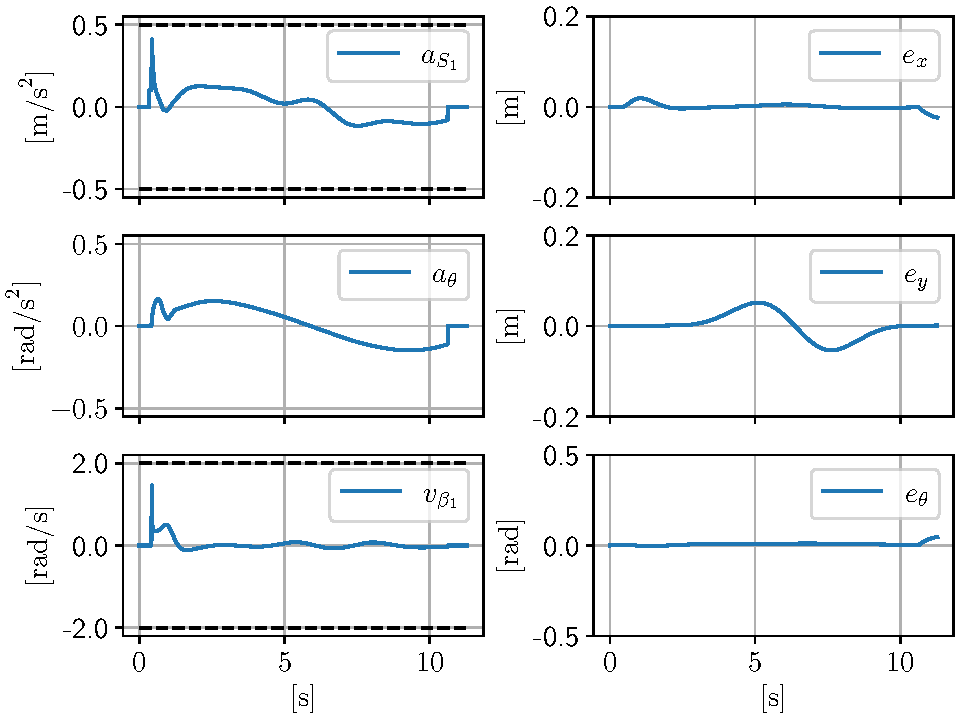
\includegraphics[width=0.75\textwidth]{figures/SWMR/simulations/circular_with_tangent_orientation/inputs_and_errors.pdf}
    \caption{Control inputs and trajectory tracking errors for the \textit{circle with tangent orientation} trajectory.}
    \label{fig:simulations:circle-with-tangent-orientation:inputs-and-errors}
\end{figure}
\begin{figure}
    \centering
    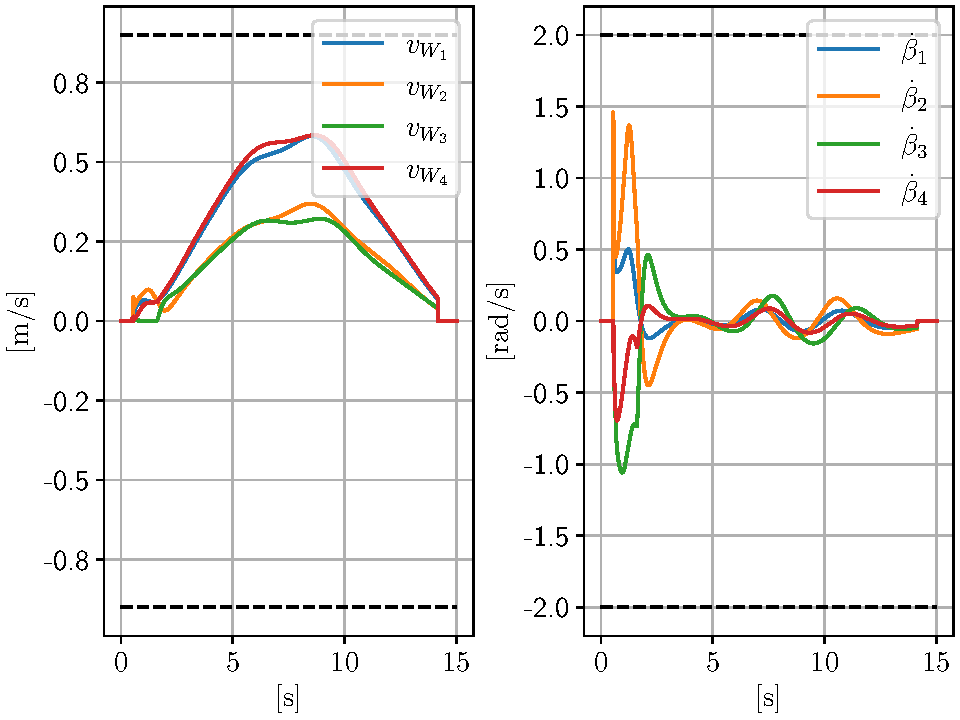
\includegraphics[width=0.75\textwidth]{figures/SWMR/simulations/circular_with_tangent_orientation/wheels_velocities.pdf}
    \caption{Driving and steering velocities of the four wheels for the \textit{circle with tangent orientation} trajectory.}
    \label{fig:simulations:circle-with-tangent-orientation:wheel-velocities}
\end{figure}

In the \textit{circle with inward orientation} trajectory, the robot is required to follow the previously defined circle, while pointing its front towards the center of the circle itself. The reference orientation is defined as
\begin{subequations}
\begin{align*}
    \theta^{\mathrm{ref}}(s) &= \mathrm{atan2}(y_C - y^{\mathrm{ref}}(s), x_C - x^{\mathrm{ref}}(s)).
\end{align*}
\end{subequations}
Here, $\theta_0=-\pi/2$ [rad], $\beta_{1,0}=\beta_{2,0}=\beta_{3,0}=\beta_{4,0}=-\pi/2$ [rad]. Moreover, $R=0.6$ [m], $\phi=\pi/2$ [rad], and $t_f=18.8$~[s].
Figure \ref{fig:experiments:circle-with-inward-orientation:snapshots} shows a sequence of snapshots of the mobile base moving while tracking the reference trajectory. In this experiment, it is possible to notice that the position of the mobile base is identical to the one of the previous section. The reference orientation, on the other hand, is such that the front of the robot points towards the center of the circle. Figure \ref{fig:simulations:circle-with-inward-orientation:inputs-and-errors} shows the control inputs computed by the NMPC and the trajectory tracking error. Figure \ref{fig:simulations:circle-with-inward-orientation:wheel-velocities} shows the corresponding driving and steering velocities.
\begin{figure*}
    \centering
    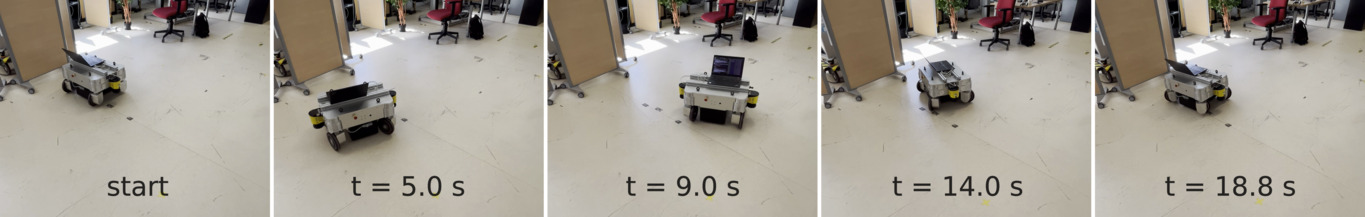
\includegraphics[width=\textwidth]{figures/SWMR/simulations/circular_with_inward_orientation/snapshots.jpeg}
    \caption{Snapshots of the mobile base tracking a \textit{circle with inward orientation}.}
    \label{fig:experiments:circle-with-inward-orientation:snapshots}
\end{figure*}
\begin{figure}
    \centering
    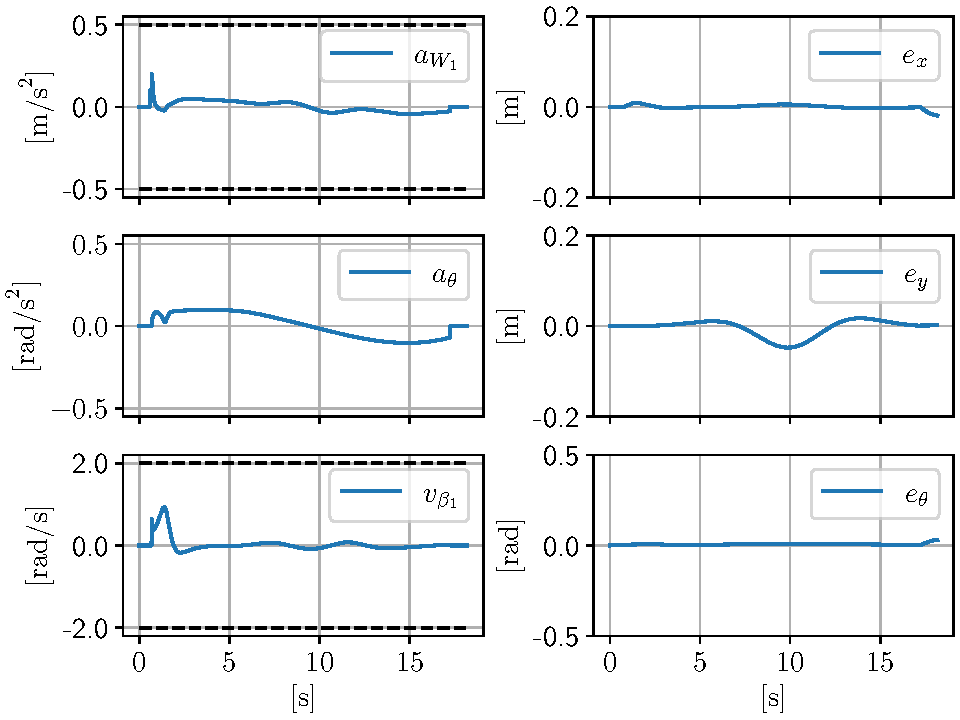
\includegraphics[width=0.75\textwidth]{figures/SWMR/simulations/circular_with_inward_orientation/inputs_and_errors.pdf}
    \caption{Control inputs and trajectory tracking errors for the \textit{circle with inward orientation} trajectory.}
    \label{fig:simulations:circle-with-inward-orientation:inputs-and-errors}
\end{figure}
\begin{figure}
    \centering
    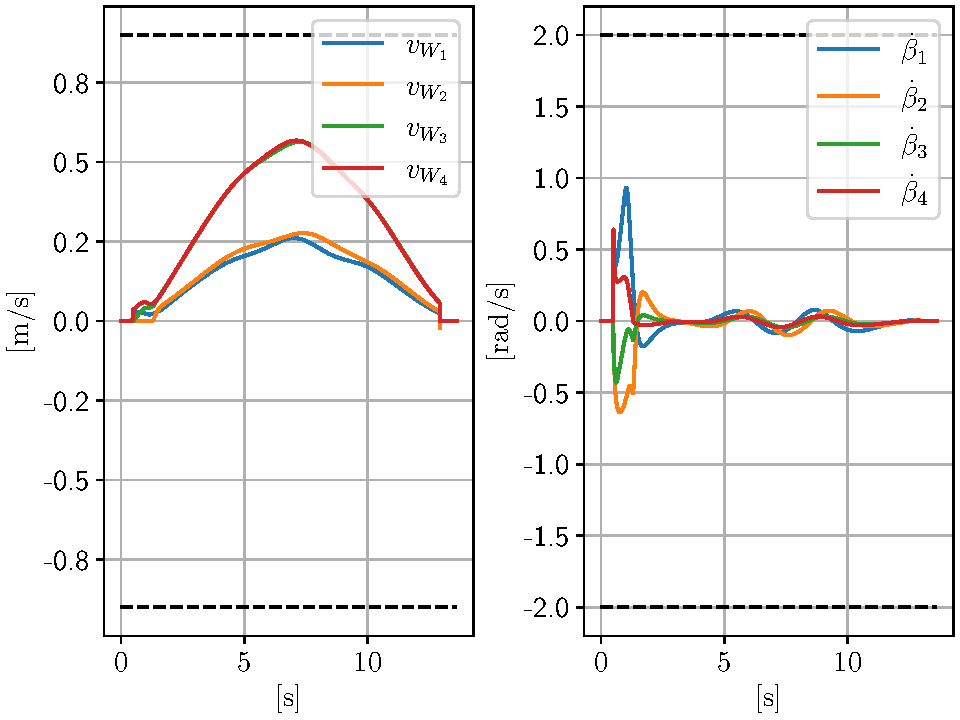
\includegraphics[width=0.75\textwidth]{figures/SWMR/simulations/circular_with_inward_orientation/wheels_velocities.pdf}
    \caption{Driving and steering velocities of the four wheels for the \textit{circle with inward orientation} trajectory.}
    \label{fig:simulations:circle-with-inward-orientation:wheel-velocities}
\end{figure}

In the \textit{circle with outward orientation} trajectory, the robot is required to follow the previously defined circle, while pointing its back towards the center of the circle itself. The reference orientation is defined as
\begin{subequations}
\begin{align*}
    \theta^{\mathrm{ref}}(s) &= \mathrm{atan2}(y^{\mathrm{ref}}(s) - y_C, x^{\mathrm{ref}}(s) - x_C).
\end{align*}
\end{subequations}
Here, $\theta_0=\pi/2$ [rad], $\beta_{1,0}=\beta_{2,0}=\beta_{3,0}=\beta_{4,0}=\pi/2$ [rad]. Moreover, $R=0.6$ [m], $\phi=\pi/2$ [rad], and $t_f=18.8$~[s]. %Figure \ref{fig:experiments:circle-with-outward-orientation:snapshots} shows a sequence of snapshots of the mobile base moving while tracking the considered trajectory. Figure \ref{fig:simulations:circle-with-outward-orientation:inputs-and-errors} show the control inputs computed by the NMPC and the trajectory tracking error. Figure \ref{fig:simulations:circle-with-outward-orientation:wheel-velocities} shows the corresponding driving and steering velocities.
%\begin{figure*}
%    \centering
%    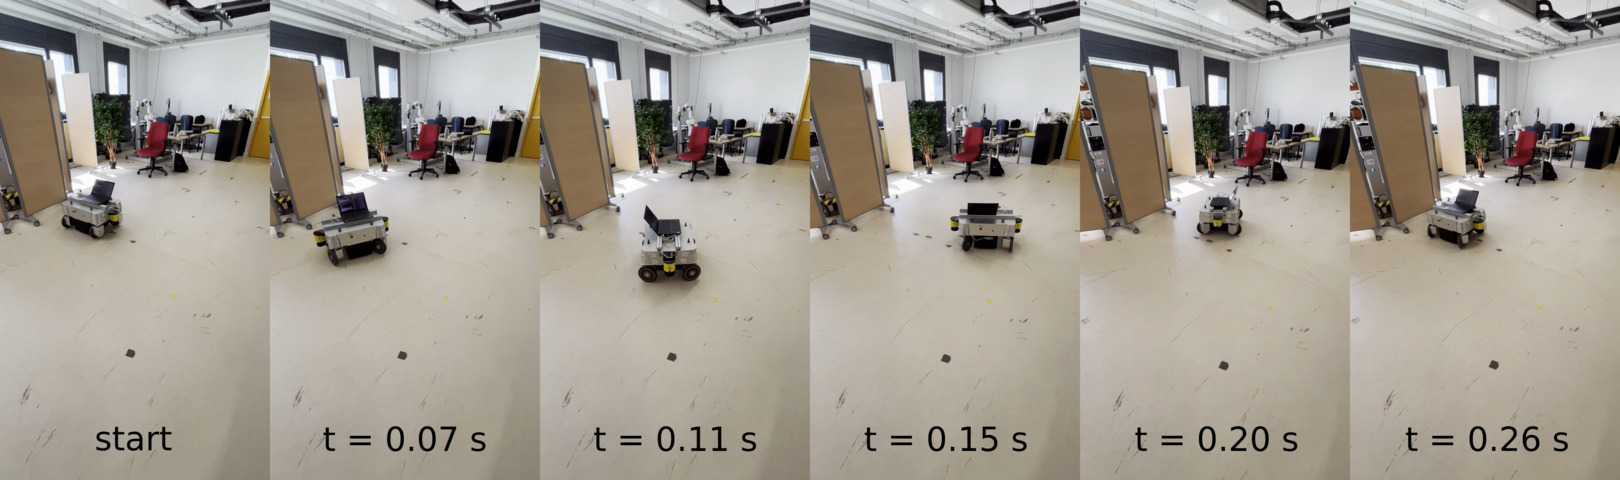
\includegraphics[width=\textwidth]{figures/SWMR/simulations/circular_with_outward_orientation/snapshots.jpeg}
%    \caption{Snapshots of the mobile base tracking a \textit{circle with outward orientation}.}
%    \label{fig:experiments:circle-with-outward-orientation:snapshots}
%\end{figure*}
%\begin{figure*}
%    \centering
%    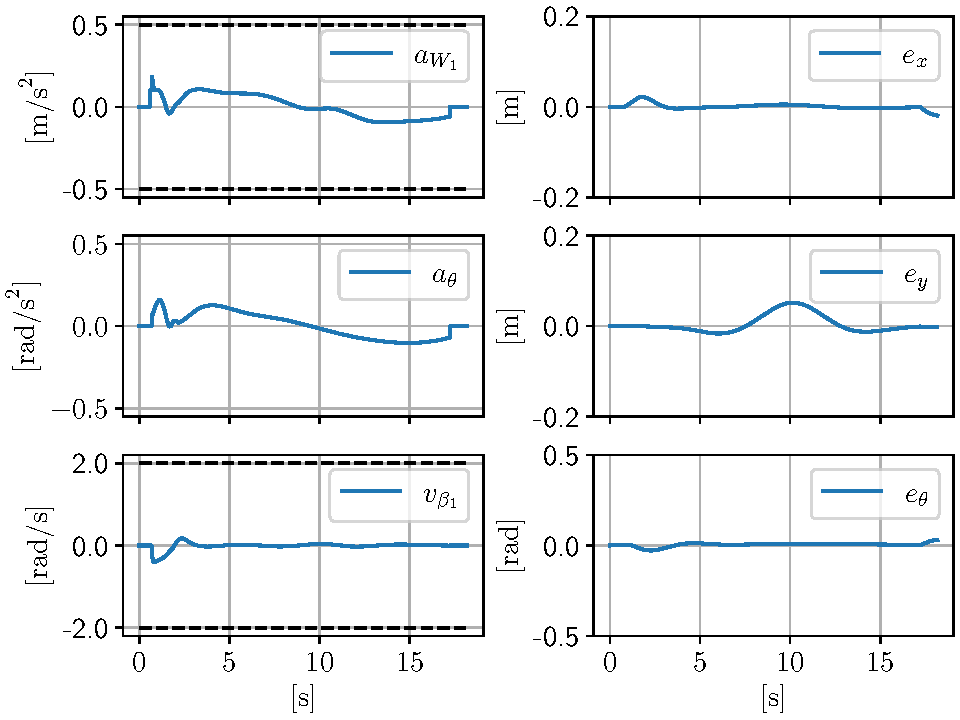
\includegraphics[width=0.8\textwidth]{figures/SWMR/simulations/circular_with_outward_orientation/inputs_and_errors.pdf}
%    \caption{Control inputs and trajectory tracking errors for the \textit{circle with outward orientation} trajectory.}
%    \label{fig:simulations:circle-with-outward-orientation:inputs-and-errors}
%\end{figure*}
%\begin{figure*}
%    \centering
%    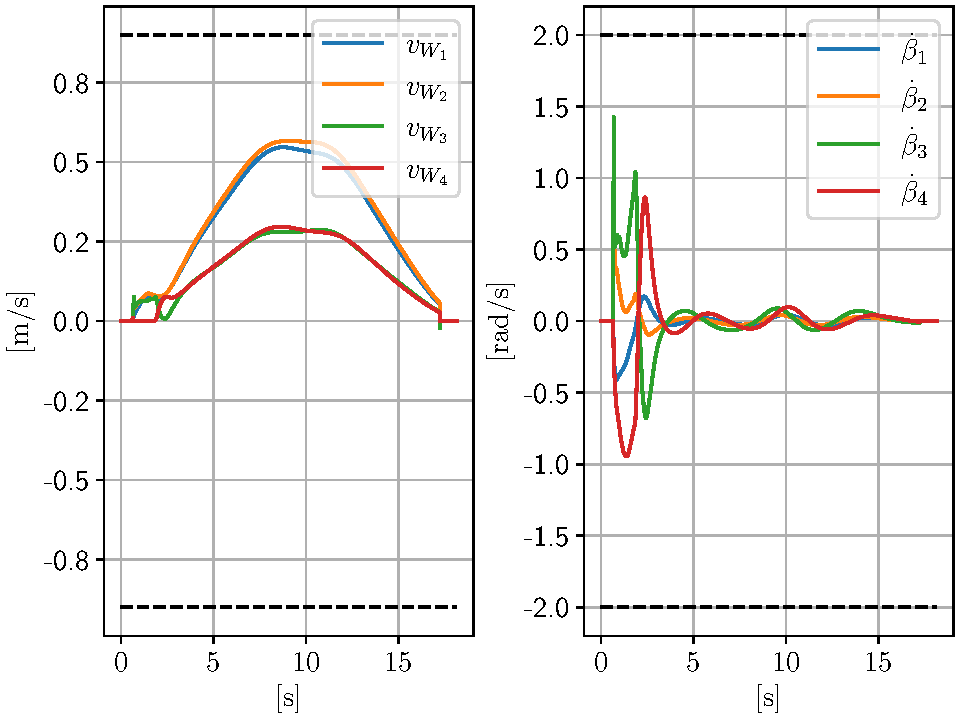
\includegraphics[width=0.8\textwidth]{figures/SWMR/simulations/circular_with_outward_orientation/wheels_velocities.pdf}
%    \caption{Driving and steering velocities of the four wheels for the \textit{circle with outward orientation} trajectory.}
%    \label{fig:simulations:circle-with-outward-orientation:wheel-velocities}
%\end{figure*}

\subsection{Slalom motions}
In this section, we consider tasks in which the robot is required to follow a sinusoidal trajectory. The reference position, which is in common among all trajectories defined below, is given by
\begin{subequations}
\begin{align*}
    x^{\mathrm{ref}}(s) &= 2 \pi s \\
    y^{\mathrm{ref}}(s) &= \alpha \sin(2 \pi s).
\end{align*}
\end{subequations}

In the \textit{slalom with constant orientation} trajectory, the robot is required to follow the above defined sinusoidal trajectory while keeping its orientation constant. The reference orientation is given by
\begin{subequations}
\begin{align*}
    \theta^{\mathrm{ref}}(t) &= \theta_0.
\end{align*}
\end{subequations}
Here, the initial orientation of the robot is $\theta_0=0.0$ [rad]. Moreover, $\beta_{1,0}=\beta_{2,0}=\beta_{3,0}=\beta_{4,0}=0.0$ [rad], $\alpha=0.8$, and $t_f=31.4$~[s].

Note that, similarly to the \textit{circle with tangent orientation}, the tracking of this kind of trajectory is only possible because of the steerable wheels.
%Figure \ref{fig:experiments:slalom-with-constant-orientation:snapshots} shows a sequence of snapshots of the mobile base moving while tracking the considered trajectory. Figure \ref{fig:simulations:slalom-with-constant-orientation:inputs-and-errors} show the control inputs computed by the NMPC and the trajectory tracking error. Figure \ref{fig:simulations:slalom-with-constant-orientation:wheel-velocities} shows the corresponding driving and steering velocities.
%\begin{figure*}
%    \centering
%    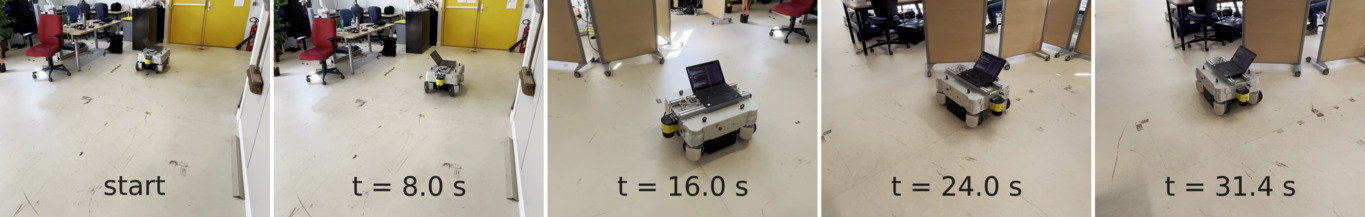
\includegraphics[width=\textwidth]{figures/SWMR/simulations/slalom_with_constant_orientation/snapshots.jpeg}
%    \caption{Snapshots of the mobile base tracking a \textit{slalom with constant orientation}.}
%    \label{fig:experiments:slalom-with-constant-orientation:snapshots}
%\end{figure*}
%\begin{figure*}
%    \centering
%    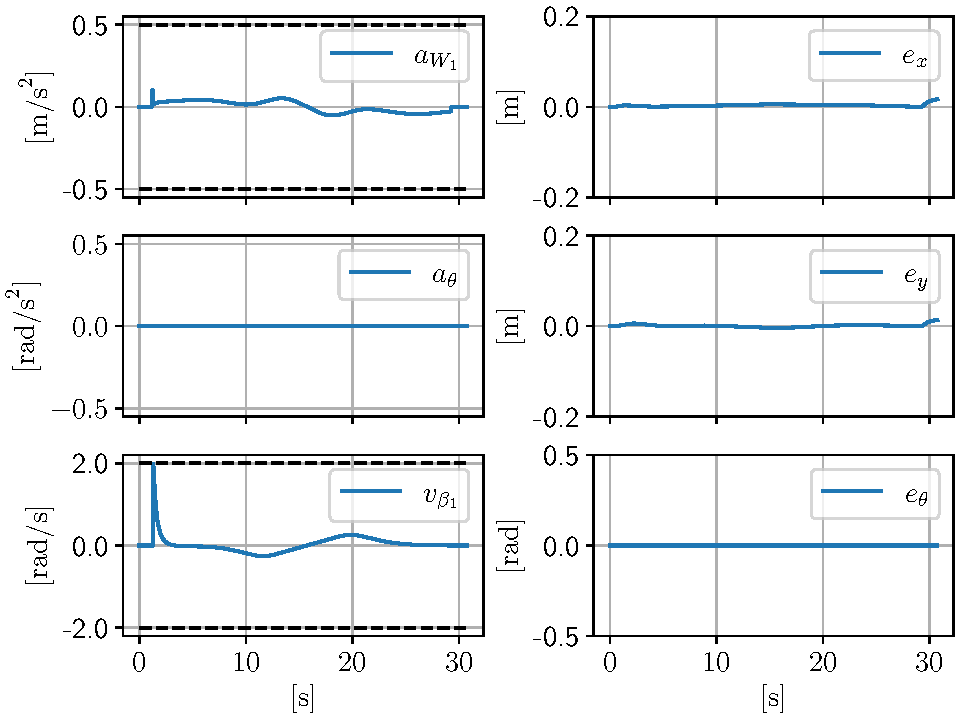
\includegraphics[width=0.8\textwidth]{figures/SWMR/simulations/slalom_with_constant_orientation/inputs_and_errors.pdf}
%    \caption{Control inputs and trajectory tracking errors for the \textit{slalom with constant orientation} trajectory.}
%    \label{fig:simulations:slalom-with-constant-orientation:inputs-and-errors}
%\end{figure*}
%\begin{figure*}
%    \centering
%    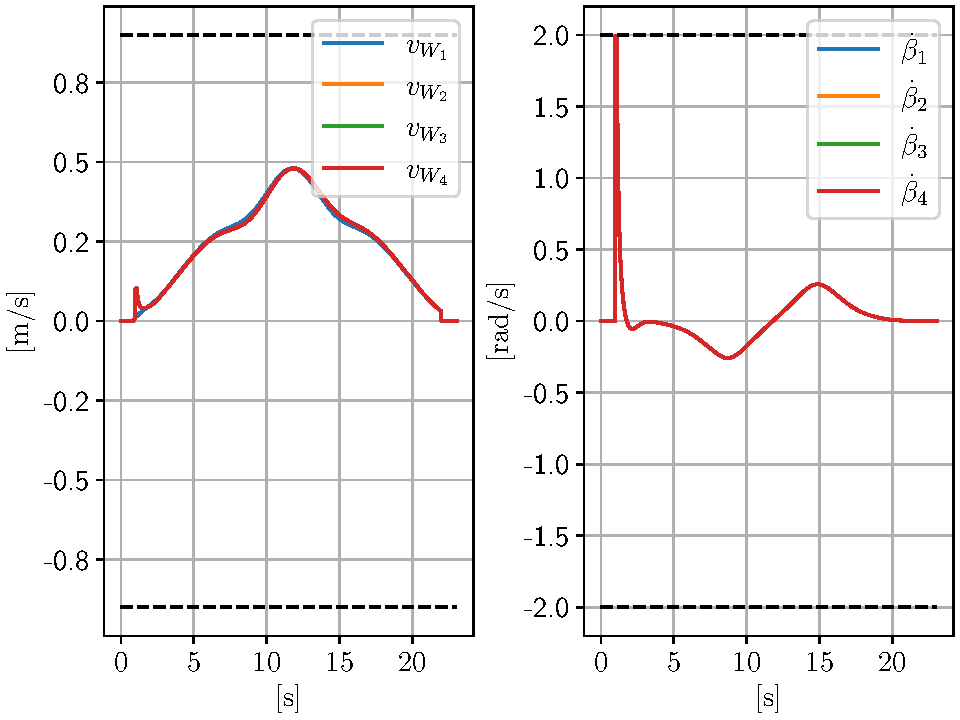
\includegraphics[width=0.8\textwidth]{figures/SWMR/simulations/slalom_with_constant_orientation/wheels_velocities.pdf}
%    \caption{Driving and steering velocities of the four wheels for the \textit{slalom with constant orientation} trajectory.}
%    \label{fig:simulations:slalom-with-constant-orientation:wheel-velocities}
%\end{figure*}

In the \textit{slalom with tangent orientation} trajectory, the robot is required to follow again the sinusoidal trajectory defined above, but while keeping its orientation tangent to the trajectory itself. The reference orientation is given by eq. \eqref{eq:reference-tangent-orientation}.
Here, the initial orientation of the robot is $\theta_0=\mathrm{atan}(\alpha)$ [rad]. Moreover, $\beta_{1,0}=\beta_{2,0}=\beta_{3,0}=\beta_{4,0}=0.0$ [rad], with $\alpha=0.8$, and $t_f=31.4$~[s].

Figure \ref{fig:experiments:slalom-with-tangent-orientation:snapshots} shows a sequence of snapshots of the mobile base moving while tracking the considered trajectory. Here, the reference position is the same as the one defined in the previous section, while the reference orientation in different. In the snapshots, it is possible to notice how the robot tracks the slalom while keeping its orientation tangent to the slalom itself. Figure \ref{fig:simulations:slalom-with-tangent-orientation:inputs-and-errors} shows the control inputs computed by the NMPC and the trajectory tracking error, which is always close to zero. Figure \ref{fig:simulations:slalom-with-tangent-orientation:wheel-velocities} shows the corresponding driving and steering velocities. Once again, the NMPC generates feasible control inputs while satisfying driving and steering velocity constraints on all wheels.
\begin{figure*}
    \centering
    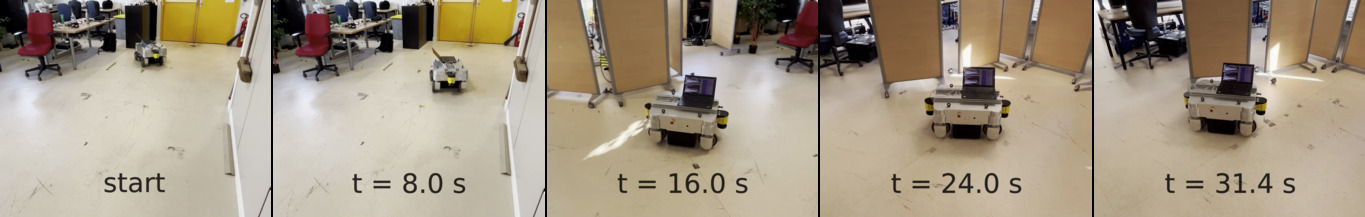
\includegraphics[width=\textwidth]{figures/SWMR/simulations/slalom_with_tangent_orientation/snapshots.jpeg}
    \caption{Snapshots of the mobile base tracking a \textit{slalom with tangent orientation}.}
    \label{fig:experiments:slalom-with-tangent-orientation:snapshots}
\end{figure*}
\begin{figure}
    \centering
    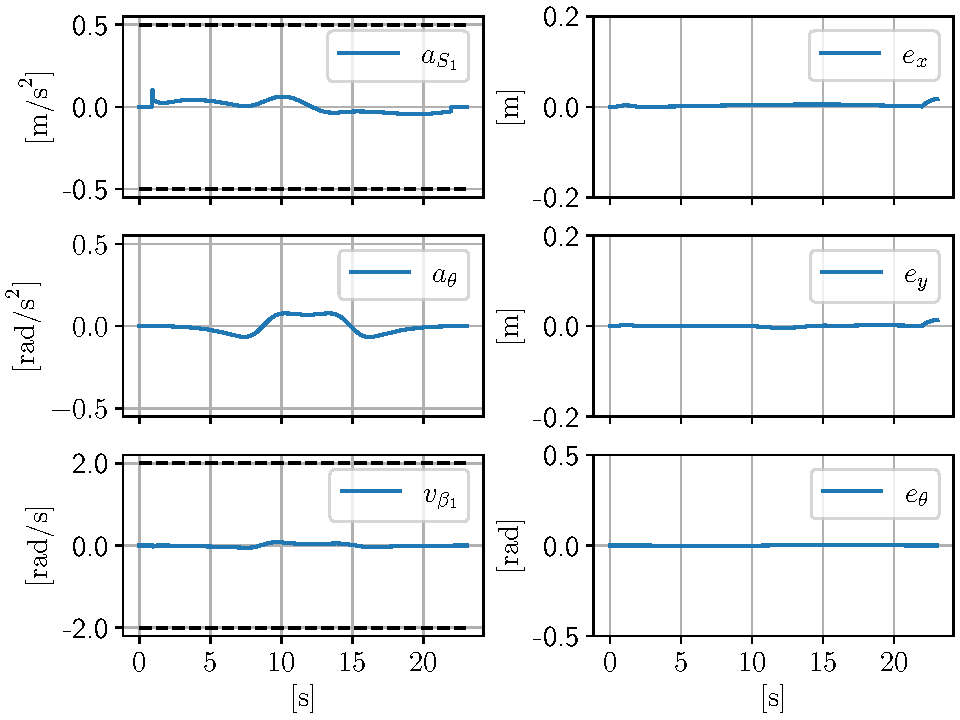
\includegraphics[width=0.75\textwidth]{figures/SWMR/simulations/slalom_with_tangent_orientation/inputs_and_errors.pdf}
    \caption{Control inputs and trajectory tracking errors for the \textit{slalom with tangent orientation} trajectory.}
    \label{fig:simulations:slalom-with-tangent-orientation:inputs-and-errors}
\end{figure}
\begin{figure}
    \centering
    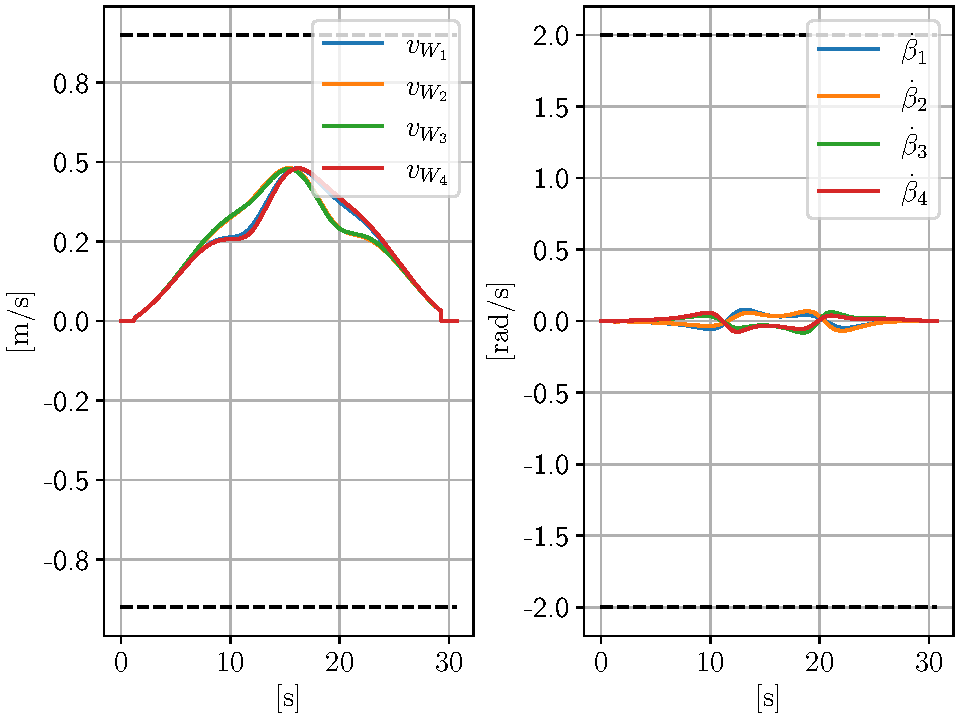
\includegraphics[width=0.75\textwidth]{figures/SWMR/simulations/slalom_with_tangent_orientation/wheels_velocities.pdf}
    \caption{Driving and steering velocities of the four wheels for the \textit{slalom with tangent orientation} trajectory.}
    \label{fig:simulations:slalom-with-tangent-orientation:wheel-velocities}
\end{figure}

\section{Conclusions}
\label{sec:conclusions}
In this work, we presented a framework for trajectory tracking with steerable wheeled mobile robots, which makes use of a Nonlinear MPC based on real-time iteration. Our scheme is capable of tracking trajectories without violating wheels' velocity constraints, while taking into account kinematic model singularities. We have validated our approach on multiple trajectories using the Neobotix MPO-700, showing that our scheme is always able to track them. To the best of our knowledge, this is the first time a NMPC has been implemented on a SWMR.

In our future works, we plan to extend the framework in several ways:
\begin{enumerate}
    \item extend the NMPC to a dual-arm mobile manipulators such as BAZAR robot \cite{Cherubini2019ACR}, making it interact with the environments with the arms while moving;
    \item implement a motion planning algorithm such as kinodynamic RRT* \cite{Webb2013KinodynamicRRTstar}, making the robot able to navigate autonomously in an environment with obstacles;
    \item further improve the performance of the framework by implementing it in C++ (while the scheme runs in real-time thanks to acados which compiles the NMPC, most of the time is taken by the auxiliary trajectory generation, which completely relies on Python).
\end{enumerate}
